\documentclass[12pt,a4paper,twoside,openright]{report}

\usepackage{amssymb}
\usepackage{rotating}
\usepackage{subcaption}
\PassOptionsToPackage{hyphens}{url}\usepackage[breaklinks=true]{hyperref}
\usepackage[acronym]{glossaries}
\usepackage{graphicx}
\usepackage[utf8]{inputenc}
\usepackage[british]{babel}
\usepackage[backend=biber,style=alphabetic,sortcites,backref,hyperref]{biblatex}
\usepackage{listings}
\usepackage{afterpage}
\usepackage{lineno}
\usepackage[left=3.0cm,right=3.0cm,top=4cm,bottom=3.5cm]{geometry}
\usepackage{titlesec}
\usepackage{caption}
\usepackage{csquotes}

\lstset{aboveskip=12pt}

%\linenumbers

\newcommand\blankpage{%
    \null
    \thispagestyle{empty}%
    \newpage}

\newcommand{\specialcell}[2][c]{%
  \begin{tabular}[#1]{@{}c@{}}#2\end{tabular}}

%% headers
\titleformat{\chapter}{\normalfont\huge}{\thechapter.}{20pt}{\huge}
\pagestyle{myheadings}
\renewcommand{\chaptermark}[1]{ \markboth{#1}{} }
\renewcommand{\sectionmark}[1]{ \markright{#1}{} }

%% bold float labels
\DeclareCaptionLabelFormat{myformat}{\textbf{#1}~\textbf{#2}}
\captionsetup{labelformat=myformat}

%% rename index with care for babel package
\addto\captionsbritish{%
  \renewcommand{\contentsname}%
  {Table of Contents}%
}

%% do not split long footnotes over multiple pages
\interfootnotelinepenalty=10000


%\title{Advances in Digital Research Repositories}
%\author{Adrian-Tudor P\u{a}nescu}

\newacronym{oa}{OA}{Open Access}
\newacronym[firstplural=Institutional Repositories (IRs)]{ir}{IR}{Institutional Repository}
\newacronym{etl}{ETL}{Extract, Transform, Load}
\newacronym{dmp}{DMP}{Data Management Plan}
\newacronym{san}{SAN}{Storage Area Network}
\newacronym{csv}{CSV}{Comma-Separated Values}
\newacronym{dicom}{DICOM}{Digital Imaging and Communications in Medicine}
\newacronym{cdisc}{CDISC}{Clinical Data Interchange Standards Consortium}
\newacronym{cdash}{CDASH}{Clinical Data Acquisition Standards Harmonization}
\newacronym{stdm}{STDM}{Study Data Tabulation Model}
\newacronym{mets}{METS}{Metadata Encoding and Transmission Standard}
\newacronym{ands}{ANDS}{Australian National Research Data Storage Services}
\newacronym{ntro}{NTRO}{Non-Traditional Research Output}
\newacronym{cerif}{CERIF}{Common European Research Information Format}
\newacronym{ddi}{DDI}{Document, Discover and Interoperate}
\newacronym{foaf}{FOAF}{Friend of a Friend}
\newacronym{mime}{MIME}{Multipurpose Internet Mail Extensions}
\newacronym{xml}{XML}{Extensible Markup Language}
\newacronym{json}{JSON}{JavaScript Object Notation}
\newacronym{isbn}{ISBN}{International Standard Book Numbers}
\newacronym{issn}{ISSN}{International Standard Serial Numbers}
\newacronym{ark}{ARK}{Archival Resource Key}
\newacronym{doi}{DOI}{Digital Object Identifier}
\newacronym{isni}{ISNI}{International Standard Name Identifier}
\newacronym{rrid}{RRID}{Research Resource Identifiers}
\newacronym{fair}{FAIR}{Findable, Accessible, Interoperable, Reusable}
\newacronym{pid}{PID}{Persistent Identifier}
\newacronym{www}{WWW}{World Wide Web}
\newacronym{rdf}{RDF}{Resource Description Framework}
\newacronym{uk}{UK}{United Kingdom}
\newacronym{acl}{ACL}{Access Control List}
\newacronym{us}{US}{United States}
\newacronym{eu}{EU}{European Union}
\newacronym{gdpr}{GDPR}{General Data Protection Regulation}
\newacronym{cc}{CC}{Creative Commons}
\newacronym{gpl}{GPL}{GNU General Public License}
\newacronym{eupl}{EUPL}{European Union Public Licence}
\newacronym{ogl}{OGL}{Open Government Licence}
\newacronym{eoa}{EOA}{Ethereum externally owned account}
\newacronym{rss}{RSS}{RDF Site Summary}
\newacronym{apc}{APC}{Article Publishing Charges}
\newacronym{oai}{OAI}{Open Archives Initiative}
\newacronym{pmh}{PMH}{Protocol for Metadata Harvesting}
\newacronym{covid}{COVID-19}{Coronavirus disease 2019}
\newacronym{uri}{URI}{Uniform Resource Identifier}
\newacronym{jsonld}{JSON-LD}{JavaScript Object Notation for Linked Data}
\newacronym{rdfa}{RDFa}{RDF in Attributes}
\newacronym{dcmt}{DCMT}{Dublin Core Metadata Terms}
\newacronym{rest}{REST}{Representational State Transfer}
\newacronym{api}{API}{Application Programming Interface}
\newacronym{xslt}{XSLT}{Extensible Stylesheet Language Transformations}
\newacronym{mods}{MODS}{Metadata Object Description Schema}
\newacronym{saas}{SaaS}{Software as a Service}
\newacronym{pdf}{PDF}{Portable Document Format}
\newacronym{cris}{CRIS}{Current Research Information System}
\newacronym{html}{HTML}{HyperText Markup Language}
\newacronym{http}{HTTP}{Hypertext Transfer Protocol}
\makeglossaries

\bibliography{thesis}
\linespread{1.3}

\begin{document}
    \pagenumbering{gobble}

    %!TEX root=../main.tex

\begin{titlepage}
  \centering
  \vspace*{\baselineskip}
  \textbf{\textit{Doctoral Dissertation}}
  \\\vspace*{\baselineskip}
  \rule{\textwidth}{1.6pt}\vspace*{-\baselineskip}\vspace*{2pt}
  \rule{\textwidth}{0.4pt}\\[\baselineskip]
  {ADVANCES IN DIGITAL RESEARCH REPOSITORIES}
  \rule{\textwidth}{0.4pt}\vspace*{-\baselineskip}\vspace*{2pt}
  \rule{\textwidth}{1.6pt}\\[\baselineskip]
  \scshape
  \vspace*{4\baselineskip}
  Candidate:
  \\\vspace*{0.5\baselineskip}
  ADRIAN-TUDOR P\u{A}NESCU
  \\\vspace*{4\baselineskip}
  Advisor:
  \\\vspace*{\baselineskip}
  \begin{minipage}{0.9\textwidth}
    \centering
    VASILE ION MANTA\\
    Faculty of Automatic Control and Computer Engineering\\``Gheorghe Asachi'' Technical University of Ia\c{s}i
  \end{minipage}
  \\\vspace*{0.5\baselineskip}
  \begin{minipage}{0.8\textwidth}
    \centering
    
\includegraphics[scale=0.7]{figures/logo.png}
  \end{minipage}
  \\\vspace*{2\baselineskip}
  \textit{Romania, 2020}
  \\\vspace*{0.3\baselineskip}
  \texttt{doi:c7st}
\end{titlepage}
    \blankpage

    \thispagestyle{empty}
%\noindent This work was fostered by the expertise of my employer, Figshare, the guidance of my supervisor, Vasile Manta, and the support of my parents, Maria and Doru-Adrian. I also express my gratitude to the Doctoral Committee and the anonymous reviewers of the supporting publications; peer review is one of the main pillars of the scientific method.
    \blankpage
    
    \begin{abstract}
        This work presents the evolution of research repositories, from collections of peer-reviewed outputs, such as journal articles or monographs, to collections holding a wide array of materials, including data sets, preprints, scientific software or protocols, based on the new realities of the scientific research endeavour. It also discusses a number of novel practical solutions to repository issues such as licencing, bibliographic record modelling, dissemination and linking, or record management and migration by employing new technologies such as linked data, blockchain, and extract, transform and load frameworks.\\\par


\noindent Această lucrare prezintă evoluția depozitelor de materiale provenite din activitățile de cercetare, de la biblioteci ce stochează publicații verificate, precum jurnale sau monografii, la colecții digitale vaste ce includ seturi de date, \emph{preprint}-uri, software științific sau protocoale, în acord cu noile realități ale domeniului cercetării. Sunt discutate soluții practice la probleme existente în acest tip de aplicație, cum ar fi licențierea materialelor, modelarea, diseminarea și corelarea informațiilor bibliografice sau administrarea și migrarea lor, soluții ce fac uz de tehnologii noi precum \emph{linked data}, \emph{blockchain} sau sisteme de extragere, transformare și încărcare.  
    \end{abstract}
    \blankpage

    \printglossary[type=\acronymtype,title=Abbreviations]
    \tableofcontents

    % ensure we start on an odd page when double-side printing
    \cleardoublepage 
    \pagenumbering{arabic}

    %\baselineskip=18pt plus1pt. % line spacing

    
    \chapter{Introduction}
        \label{ch:intro}
        Libraries, structured and curated collections of informational resources, play a key role in preserving the collective memory of the human civilisation and its heritage. The resources they store take various structural (manuscripts, media, articles) and semantic (historic records, research, literature) forms and are made available to either the general public or more finer-grained user groups.

With the advent of the \gls{www} in the late 20th century, libraries were among the first applications of the new online technologies, giving rise to \emph{digital} libraries. It can be argued that the \gls{www} as a whole represents in itself a library; still, discrete instances can maintain the structural and semantic differentiation mentioned previously and can better target various user groups, catering to their specific needs.

As the \gls{www} was the driving factor behind the digitisation of libraries, the progress of scholarship and scientific research played an important role in the evolution of digital libraries, a number of aspects being factored into this. First, research funding has greatly increased, as presented in Fig. \ref{fig:fundig} and, as a direct result, the number of outputs, such as monographs, journal articles or theses, has increased (see Fig. \ref{fig:nopublications}). This impacted digital libraries which now need to be able to manage a larger influx of new content while ensuring its proper dissemination across stakeholders. 
\begin{figure}[ht!]
\centering
\begin{subfigure}{0.9\textwidth}
  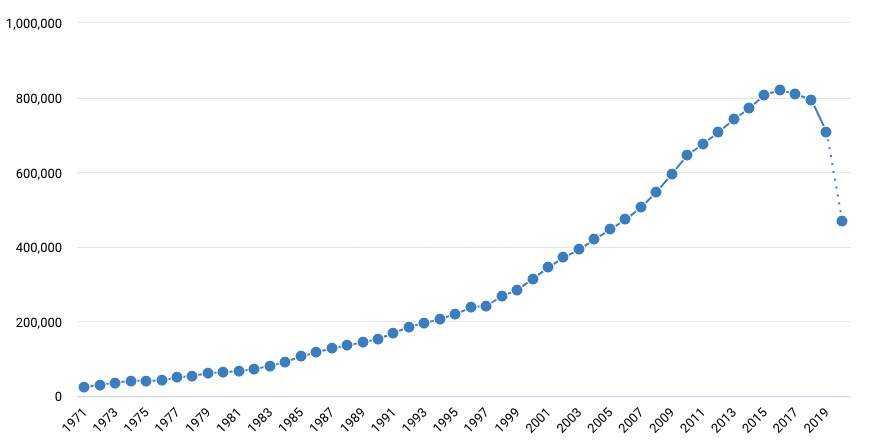
\includegraphics[width=1\linewidth]{figures/no_grants.png}  
  \caption{Evolution of number of research grants since 1971. Data since 2018 is incomplete.}
  \label{subfig:grants}
\end{subfigure}
\begin{subfigure}{0.9\textwidth}
  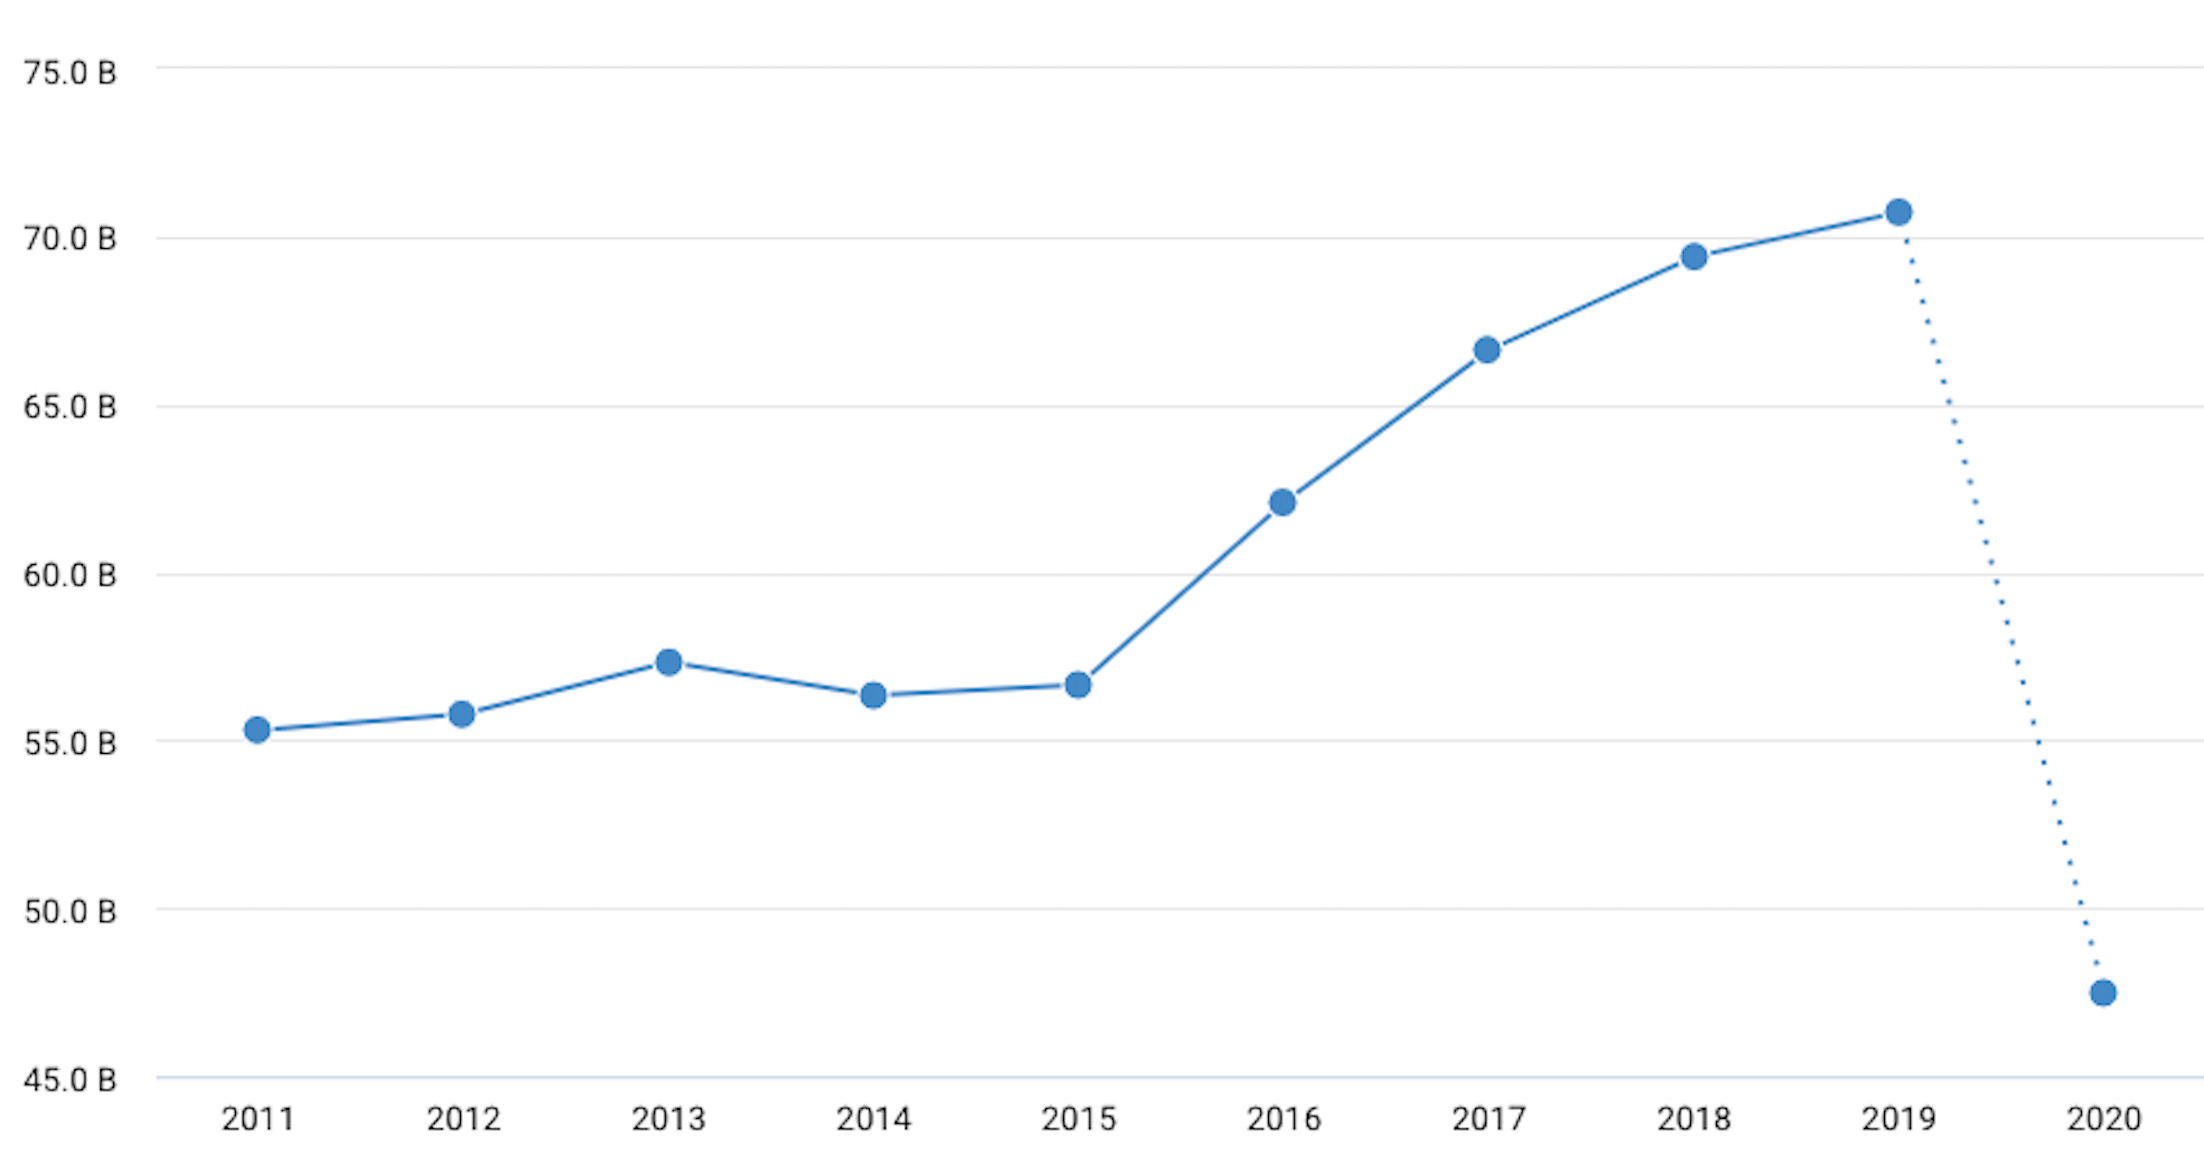
\includegraphics[width=1\linewidth]{figures/funding.png}  
  \caption{Evolution of total amount of research grants since 2011, in pounds sterling. Data for 2020 is incomplete.}
  \label{subfig:grantstotal}
\end{subfigure}
\caption{Evolution of research funding; source \url{https://app.dimensions.ai}.}
\label{fig:fundig}
\end{figure}

\begin{figure}[ht!]
\centering
  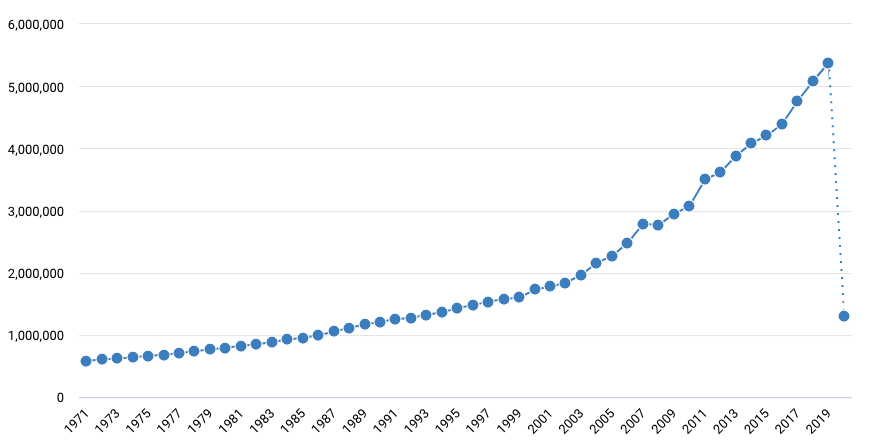
\includegraphics[width=1\linewidth]{figures/publications.png}  
  \caption{Evolution of number of research publications, data since 2019 is incomplete; source \url{https://app.dimensions.ai}.}
  \label{fig:nopublications}
\end{figure}

Second, a number of significant events in the area of research and scholarly communications have taken place; two of these are of interest.

The \emph{\gls{oa}} reforms came to prominence along with digital libraries; as the medium for disseminating research switched from physical (paper journals or monographs) to digital, researchers questioned the suitability of the traditional business plans of publishers (e.g., Springer Nature or Elsevier), which could no longer fully justify the costs inquired for typesetting and printing, among others. \gls{oa} is one proposed way of resolving this, its aim being to shift the costs of publishing from being supported by consumers to being supported by producers (i.e., researchers wishing to disseminate their work, or, most often, their funders). \gls{oa} can be practically implemented in a number of ways, but of interest here are the following:
\begin{itemize}
    \item Gold: the article is published as \gls{oa} in a journal pending the publication of a fee by the authors and using a licencing model that places no barriers towards sharing and reuse.
    \item Green: while the reviewed, typeset and copy-edited article is published by the journal under its own terms, the authors are allowed to freely share their own versions using other means.
\end{itemize}
An obvious platform for depositing both these types of \gls{oa} manuscripts is the digital library managed by the authors' affiliated institutions. In \cite{oa} the authors measured that between 2000 and 2016 over 4 million gold \gls{oa} have been published and over 2 million green \gls{oa} versions have been deposited in repositories.

\gls{oa} is a subset of a much complex movement, \emph{open science}, which aims at making all research outputs and workflows publicly available; this includes, but is not limited to, tools and applications used in research, methods for measuring the impact of published results, or policies allowing a wider audience to consume and produce research\footnote{An example here is the concept of \emph{citizen science}, which aims at involving amateurs in research by allowing them, among others, to perform repetitive task which do not require in-depth domain knowledge.}.

The \emph{reproducibility crisis} is a phenomenon generated by a number of research studies that failed to \emph{replicate}, other researchers not being able to verify the claims of the original authors by repeating similar experiments. An infamous such example is a paper\footnote{Wakefield et. al. (1998) \emph{RETRACTED: Ileal-lymphoid-nodular hyperplasia, non-specific colitis, and pervasive developmental disorder in children}} published in 1998 in The Lancet, which linked the measles, mumps and rubella vaccine to colitis and autism spectrum disorders in children. The paper was lately retracted, due to evidence of fraud, conflicts of interest and manipulation of data. The literature currently documents multiple instances of studies that exhibit reproducibility or replication\footnote{It is widely accepted that \emph{reproducibility} is the act of reaching original research result by using the same research materials (data, software, instruments), while \emph{replicability} uses different inputs (e.g., a new set of patients for a clinical study) in order to reach similar results\cite{patil}.} issues, due to, among others, technical, methodology or workflow faults (see, for example \cite{eklund,seekblastn}).

As a result of this crisis, the world of research focused in latest years on ensuring that published scientific result are accompanied by all the required artefacts (e.g., data, software, protocols) necessary to allow other researchers to fully verify the claims of the original authors. This move was also formalised by both research funding bodies\cite{h2020,nih} and publishers\cite{scidat,elsdat}, such that good practices are enforced across the whole scientific community. This type of policies are part of the \emph{open data} movement, which along with \gls{oa} form the so-called \emph{democratic} school of thought in open science, which concerns itself with removing any barriers to accessing and reusing research.

For digital research libraries this meant, above everything, adapting to the new types of outputs; data sets or scientific software present new challenges, due to their structural and semantic particularities. Moreover, libraries need to ensure that all outputs generated by a scientific study are presented in a coherent and consolidated manner, in order to facilitate reproducibility. Assisting with reproducibility is a crucial dimension that needs to be considered by \emph{all} tools in the research ecosystem, as \emph{``expecting a researcher to reproduce either entirely or in part the outcomes of a large or costly study or data collection exercise is not reasonable''}\cite{oa} and thus, all possible forms of assistance, including those at the technological level, need to made available.

In \cite{oa} the authors note that \emph{``the reproducibility crisis is just one manifestation of a broken credit system where researchers are incentivised to publish positive results and suppress or disregard negative results''}; this comes to strengthen the motivations behind open science, and at the same time, suggests that the role of repositories is continuously expanding to include, for example, support for new types of outputs or novel methods of quantifying and qualifying the impact of research.

This thesis documents the evolution of digital libraries in light of the two challenges mentioned above and by describing how this suite of applications has overcome them by developing new features and workflows. It approaches this by considering the development of \emph{data repositories}, digital libraries aimed of hosting the new types of outputs mentioned above in general and research data in particular. For a considerable span of time, data repositories evolved in parallel with their more traditional counterparts, \glspl{ir}, archives of intellectual outputs of a research institution, most often a university. \glspl{ir} are a subset of digital libraries, as the latter could also hold content which is not scientific in nature, and, as opposed to data repositories, are more focused on scientific \emph{literature}, such as journal articles, monographs or theses. It is worth noting that across the thesis the term \emph{repository} is employed, due to its wide use in the field as a direct result of the spread of \gls{ir} solutions.

Nevertheless, in the last years, institutional, data, software and other scientific outputs repositories started to converge into unified solutions which can accommodate the disparate needs of researchers on one hand, and minimise the administrative work of librarians and technology teams on the other\footnote{The distinction between this two types of staff is beginning to fade, as librarians need to adapt to the new realities of the research ecosystem by including software-assisted workflows and tools in their craft; an example of this is the the Software Carpentry project at \url{https://software-carpentry.org/blog/2015/05/coding-for-librarians.html}.}. Thus, it can be argued that a new type of platform, the \emph{research}, or, as \cite{cmu} designates it, \emph{comprehensive} repository is beginning to take shape, by taking advantage of both the strong points of each type of existing platform, and also of the opportunities offered by the new research ecosystem and evolution of technology in general.

Thus, Chapter \ref{ch:evolution} begins with a detailed description of data repositories and follows with a description of the reasons and means for merging all types of repository applications into generic research repositories. The next three chapters focus on the practical implementation of features and workflows which could benefit this type of software infrastructure, namely licencing solutions using blockchains and smart contracts (Chapter \ref{ch:blockchain}), data modelling using \gls{rdf} (Chapter \ref{ch:rdf}), and record migration and management solutions employing \gls{etl} pipelines. This is an attempt of employing tools and processes specific to software engineering, which are wide spread in other types of applications, to digital libraries, with the aim of presenting a possible blueprint for the next generation research repository.

    \chapter{From institutional to research repositories}
        \label{ch:evolution}
        One of the first definitions of an \gls{ir} is \emph{``a set of services that a university offers to the members of its community for the management and dissemination of digital materials created by the institution and its community members. It is most essentially an organisational commitment to the stewardship of these digital materials, including long-term preservation where appropriate, as well as organisation and access or distribution. While operational responsibility for these services may reasonably be situated in different organisational units at different universities, an effective institutional repository of necessity represents a collaboration among librarians, information technologists, archives and records managers, faculty, and university administrators and policymakers. At any given point in time, an institutional repository will be supported by a set of information technologies, but a key part of the services that comprise an institutional repository is the management of technological changes, and the migration of digital content from one set of technologies to the next as part of the organisational commitment to providing repository services. An institutional repository is not simply a fixed set of software and hardware.''}\cite{lynch}.

This extensive definition is interesting for a number of reasons. First, it places the repository in the context of an \emph{institution}, an organisation that has \emph{research} as its main object of activity. As a result, it is used for managing \emph{all} outputs that are a result of research; for example, here are three repositories used by universities for managing their scholarship:
\begin{itemize}
    \item DSpace@MIT, the digital repository of the Massachusetts Institute of Technology: \url{https://dspace.mit.edu/}
    \item VTechWorks, the scholarship access platform of Virginia Tech: \url{https://vtechworks.lib.vt.edu/}
    \item ORA, the Oxford University Research Archive: \url{https://ora.ox.ac.uk/}
\end{itemize}

Second, the definition enumerates the three main functions a repository needs to implement:
\begin{enumerate}
    \item Stewardship and organisation: as mentioned in the introduction, repositories are the digital equivalent of physical libraries and, as a result, they need to implement most of the workflows and practices in this area. These include, for example, cataloguing (creating extensive descriptions of the stored content), content classification, or curation.
    \item Preservation: traditionally libraries have ensured that the content they hold remains available over time, and in some cases this requires creating special physical environments necessary for maintaining fragile materials. While digital content might not be afflicted by the exact same issues (e.g., degradation of paper over time), special care is still required in order to ensure that it will remain available in perpetuity. 
    \item Dissemination: scholarship's value increases as the audience it reaches increases; thus it is important that repositories incorporate functionality that will facilitate the distribution and discoverability of content.
\end{enumerate}

As a direct result of the mentioned functions, the definition also mentions that repository staff needs to include not only librarians, but also information technology staff, archivist, researchers, or administrative personnel. In \cite{cmu} the authors describe a repository team comprising of over ten members in three different squads, each serving a different role in the operation of the digital library, from management, to curation, and engagement. Apart from the human resource angle, the repository does not need to be understood as a stand-alone system, but as a collection of modules, each focusing on a specific part of the encompassing workflow and providing a certain functionality to the stakeholders.

Coming back to the presented definition, the most interesting aspect in the context of this work is that it does not explicitly mention the types of content repositories should hold. The author of the cited paper elaborates on this, by making a distinction between \emph{scholarly publishing}, which is concerned, for example, with journal articles or monographs, and \emph{scholarly communication}, which is characterised by the development of new types of output, such as datasets or research software. In fact, scholarly publishing is a subset of scholarly communication, being concerned only with the specific types of outputs characteristic to \emph{traditional} research publishing.

While this definition, including the distinction above, was proposed in 2003, it is important to note that most institutional repositories focus on outputs specific to scholarly publishing (this is also true for the three repositories enumerated above). Nevertheless, the rapid evolution of scholarly communication, fuelled by \gls{oa} and the reproducibility crisis, led to the expansion of the traditional institutional repository in order to allow for the full set of scholarly communication outputs to be part of the managed corpus.

One way to look at this expansion is by considering an intermediate step between traditional institutional repositories and research repositories, namely repositories solely aimed at outputs outside the established publishing model; prime examples are data and research software repositories. Section \ref{sec:data} will take an in-depth look at data repositories while Section \ref{sec:research} will consider how data and institutional repositories merged, creating new systems which aim at managing any scholarly communications output.

\newpage

\section{Data repositories}
\label{sec:data}

Research data repositories have come to prominence as a direct result of the reproducibility crisis, as funders and publishers required researchers to publish all underlying materials along with publications and thus, platforms that could support the new types of outputs were in demand. Apart from the reproducibility crisis, it is worth noting that the scientific endeavour also evolved, researchers producing a wide array of new types of outputs, which traditionally were not published; this means that for a considerable amount of outputs researchers could not receive any credit (review from peers, citations), diminishing the usefulness of the full research activity. An interesting example of such a \gls{ntro} are \emph{negative results} which are generated by experiments, studies or analyses that did not render the expected outcomes; outputs from such endeavours crossed the line between traditional and non-traditional research publishing, as journals dedicated to negative results were established (for example, the Journal of Pharmaceutical Negative Results\footnote{\url{http://www.pnrjournal.com/}}.

As a result, a wide array of data repositories were built, either by non-profit organisations or by private companies capitalising on the new opportunities in the research ecosystem; some examples include:
\begin{itemize}
    \item ZENODO, \url{https://zenodo.org}: a public repository financed by the European Commission
    \item Dryad Digital Repository, \url{https://datadryad.org}: a non-profit repository offering paid curation and preservation services
    \item Figshare, \url{https://figshare.com}: a commercial solution with a free tier for public research
    \item Mendeley Data, \url{https://data.mendeley.com}: a repository solution developed by Elsevier, an academic publisher
    \item PANGAEA, \url{https://pangaea.de}: a data repository targeting the earth and environmental science community
\end{itemize}

As the number of options increased, both researchers and librarians faced the challenge of making the correct choice for publishing research data. This choice depends on a high number of dimensions, spanning both the facilities offered by each repository solution and the legal, policy, and technical requirements of the various stakeholders (researchers, curators funders). A common subset of these can be grouped in three main themes, storage and preservation, metadata, and legal requirements.


\subsection{Data storage and preservation}
\label{subsec:storage}

While data storage has a long history, closely linked to that of computing, research data presents a handful of new and unique challenges, especially when it comes to persistence and privacy. Most often the underlying technology for storing data can be of less relevance for the scholarly and scientific pursuit, but other characteristics can play an important role when choosing a solution.

The first considered aspect is the physical location of the data storage solution. Storing data on a local machine is advantageous as it allows the researcher to quickly access it, but might place obstacles when attempting to share it with a larger team, and also requires that the owner of the machine is fully responsible for its durability. Storage facilities managed at the institutional level, such as \gls{san} systems, move the burden of managing data storage from the individual researcher to specialised personnel, providing higher reliability and enhanced possibilities for sharing data among peers.

Nevertheless, the most common solution nowadays is for data to  be stored off-site in specialised facilities; this model became prominent with the advent of \emph{cloud} systems, such as \gls{aws}, Microsoft Azure or \gls{gcp}, and has benefits in terms of reliability, scalability and accessibility. This might be preferred when the individual researcher or institution does not possess the required resources for managing a storage solution, when large quantities of data need to be stored, or when data needs to be shared across a large network of collaborators. At the same time, the privacy and legal implications need to be considered, given that a 3\textsuperscript{rd} party usually handles the storage. It is worth noting that \emph{cloud} deployments can also be managed by governmental bodies or similar official entities, this alleviating some of the legal issues (for example, the \gls{ands}\footnote{\url{https://www.ands.org.au/}} provides such facilities to researchers in Australia, including storage of sensitive data, such as clinical trial datasets).

From a technical point of view, the choice of a storage solution needs to account for the following:
\begin{itemize}
    \item Redundancy: as no storage system can be guaranteed to function without faults it is important that data is copied and stored on different systems simultaneously. The higher the number of copies and the broader their geographical distribution, the higher the guarantee for their persistence is.
    \item Persistence: simply having data stored on a medium does not provide guarantees that, over time, it would not become inaccessible. For example, both tape drives and hard disks can become demagnetised, hence corrupting the stored data. This phenomenon is frequently described as \emph{bit rot}. Hence, data needs to be periodically tested, and if problems arise, fixed. A common method for detecting issues employs so-called \emph{checksums}, fingerprints of data files which change when even one byte switches value. If a file is detected to have changed it is usually replaced with a redundant copy.
    \item Transformation: as technology evolves, so do the methods for storing data, this also leading to deprecation; for example, floppy disks are rarely used nowadays, despite being ubiquitous just a few years back. Storage and archival systems need to account for this and migrate data to current technological requirements, while ensuring that its contents are not semantically modified.
\end{itemize} 

The second aspect of data storage relates to the employed file formats. While these will most often be enforced by various laboratory instruments and software used for producing and processing data, it is usually beneficial to apply transformations in order to ensure persistence, ease of use, and the possibility for others to work with the data; the decision on formats depends upon multiple considerations.

A first consideration is represented by the choice between proprietary and \emph{open source} file formats. Proprietary formats place a barrier for other collaborators that need to access the data file, as they might require special software or even hardware licences in order to read and modify these; for example, the Microsoft Office formats for storing tabular data (Excel files such as XLS and XLSX), can be opened only by certain applications, while \gls{csv} files can be manipulated by any text editor.

Another point relates to the standardisation of formats; file formats which are backed up by an established standard provide higher guarantees in terms of accessibility and preservation over time, as clear rules on how data is encapsulated and structured are defined. For example, the \gls{dicom} format is the \emph{de facto} method for storing and transmitting medical information; using it guarantees that any systems that implements the standard can fully read the data files. Similarly, the \gls{cdisc}\footnote{\url{https://www.cdisc.org/}} has developed a number of standards encompassing the whole research workflow, such as the \gls{cdash}, which establishes data collection procedures, or the \gls{stdm}, a standard for clinical data organisation and formatting. As a counter-example, the \gls{csv} format does not have complete standards behind it, and thus, particularities can arise at both the structural and semantic levels.
    
Finally, the effects on the research life cycle need to be considered. Producing data files is most often only the first step in the research workflow. Data files will need to be processed, shared with peers, and published alongside other outputs, such as journal articles. While it is highly improbable that data will maintain the same format along the whole cycle (published data rarely includes the whole initial raw dataset), informed choices can aid the process.

The third aspect to be considered relative to research storage choices relates to the overall structure of datasets; for example, while a single file is a more facile method for storing a data set, issues will arise when it grows in size and it needs to be processed or transferred to other systems. Similarly, a large number of files can pose issues with navigating and understanding the structure.

Large dataset instances, especially those exceeding one terabyte, might prove difficult to handle. Consider, for example, the need to transfer such a large file over the network and the possibility that the connection will drop during the operation; most often the transfer will need to be restarted, wasting the effort\footnote{Even over a fiber-optic connection one terabyte of data will require over one hour to transfer.}. In such cases, splitting the dataset might prove to be a better solution, as each smaller file can be transferred individually and independently of the others, network issues requiring only the re-transfer of unsent files. A number of storage systems include an option for so-called \emph{chunked} or \emph{multi-part} file transfers, where the system automatically splits larger files in smaller blocks, allowing these to be transferred independently, in any order, and at any point in time.

In cases where a large number of files constitute a dataset it is important to describe the overall structure such that other applications or users can understand it. Traditionally, \emph{folders} are used for categorising and structuring content, but these can prove ineffective in describing the full organisation, and certain storage systems might not even implement this facility. A common solution to this issue is including separate file(s) describing the structure, usually called \emph{manifests}, along with the actual dataset files. Preferably these would follow a standard structure and semantics, and for this purpose standards such as BagIt\footnote{\url{https://tools.ietf.org/html/draft-kunze-bagit-16}} and \gls{mets}\footnote{\url{https://www.loc.gov/standards/mets/}} have been established. Along with the structural description, these files can also contain technical information (e.g., checksums) that might ease other processes along the scholarly workflow.

An important distinction to consider, especially in the context of research repositories, is the one between storage and preservation. Preservation is a more involved process than simply ensuring that information is stored physically, being also concerned, as already alluded, with maintaining the integrity of the data, transforming it in order to ensure that it can still be consumed in line with the technological and social realities, and providing sufficient information on the data and its context such that new users can understand its purpose. All three points, and especially the latter, rely on \emph{metadata}, which documents various syntactic and semantic aspects of the underlying dataset; the next subsection provides a detailed description.

\newpage

\subsection{Metadata and identifiers}
\label{subsec:metapids}

Storing research data can have many purposes, from facilitating study replication to allowing further hypotheses to be tested. Nevertheless, archiving only the data points, with no information regarding their purpose, provenance or collection method will exponentially decrease their value over time, as both other researchers and the authors of the data will find impossible to reuse them without further information about the syntax and semantics.

Metadata, \emph{data about data}, is the information created, stored and shared in order to describe objects (either physical or digital), facilitating the interaction with said objects for obtaining knowledge\cite{niso}. Metadata can describe various aspects of the underlying data set, and it is often useful to split the various attributes based on their purpose.

\emph{Descriptive} metadata, such as the title, creators of the dataset, or description, is useful for allowing other users find and achieve a basic understanding of the dataset. Often linked to this is the \emph{licencing and rights} metadata that describes the legal ways in which the data can be shared and reused; it includes the copyright statement, rights holder and reuse terms.

\emph{Technical} metadata, which most often includes information on the data files, such as their formats and size, is useful for transferring and processing data across systems and its general management. \emph{Preservation} metadata will often enhance the technical attributes by including information useful for ensuring that data remains accessible and usable, such as the checksum or replica replacement events. Finally, \emph{structural} metadata describes the way in which data files are organised, and their formats.

Given its complexity, producing metadata can become a significant undertaking, its complexity exceeding even that of the underlying data in certain cases. This is one of the reasons for which the standardisation of metadata has become mandatory, this happening at three main levels.

At the structural level, standardisation ensures that on one hand, a minimum set of attributes is always attached to data sets and, on the other, that enough attributes are present for ensuring proper description of any possible artefact, no matter its origin, subject area, or geographical location. Multiple such standards have been developed, from more succinct ones, such as the DataCite Schema\footnote{\url{https://schema.datacite.org/meta/kernel-4.1/}} or \gls{dcmt}\footnote{\url{https://www.dublincore.org/specifications/dublin-core/dcmi-terms/}}, to more extensive, such as MARC21\footnote{\url{https://www.loc.gov/marc/bibliographic/}} or the \gls{cerif}\footnote{\url{https://www.eurocris.org/cerif/main-features-cerif}}. The usage of these standards might vary across subject areas (e.g., the \gls{ddi}\footnote{\url{https://www.ddialliance.org/}} standard is targeted at survey data in social, behavioural, and health sciences) or the main purpose of the metadata (e.g., the \gls{mets} standard emphasises technical, preservation and structural metadata more than the DataCite schema).

At the semantic level, the focus is on ensuring that the language used for describing data observes a controlled variability both inside a research area and across domains. For example, the CRediT vocabulary\footnote{\url{https://casrai.org/credit/}} defines various roles involved in research activities (analyst, investigator, publication author, etc.), \gls{foaf}\footnote{\url{http://xmlns.com/foaf/spec/}} establishes the terminology for describing and linking persons, institutions and other entities, and the \gls{mime}\footnote{\url{https://tools.ietf.org/html/rfc2046}} standard defines the various file formats.

The third point considered from a standardisation point of view involves the formats used for storing and transferring metadata. The \gls{xml}\footnote{\url{https://www.w3.org/XML/}} is one of the most prevalent formats, almost all standards providing a schema and guidance on employing it. The \gls{json}\footnote{\url{https://www.json.org/}} format is also starting to gain traction, both due to its pervasiveness in web services nowadays, and also due to certain initiatives, such as \url{schema.org} which use it as the de facto output format.

One important aspect of metadata, considered by most standards, vocabularies and formats relates to the usage of identifiers. Similar to social security numbers for persons or serial numbers for devices, when it comes to research data the aim of identifiers is to uniquely and \emph{persistently} describe it. This has become a stringent necessity in the age of internet, both due to the requirement to maintain resources accessible for periods of time of the order of years or even decades, no matter the status or location of the system preserving them at any discrete moment, and also due to the necessity of linking various resources across systems. Similar to bit rot, link rot describes the phenomenon of web addresses becoming unavailable over time, for example due to servers going offline. This can pose significant issues for research artefacts, which need to remain available for longer periods of time due to their societal importance; nevertheless, link rot was proven to be pervasive across scholarly resources\cite{sanderson}, As a result, various elements of research data started receiving identifiers, various initiatives and standards becoming available. The importance of the persistence aspect is marked by the use in the community of the \gls{pid} term.

Even before the prevalence of research data sharing, bibliographic records received identifiers, such as \gls{isbn} for books and \gls{issn} for periodicals. For research data, \glspl{ark} and Handles\footnote{\url{http://handle.net/}} are more prevalent, as these mechanisms facilitate issuing new identifiers and thus, are more suited for the larger volume of produced records.

The \gls{doi} system\footnote{\url{https://doi.org}} is quickly emerging as the industry standard; it builds upon the Handle infrastructure, but adds an additional dimension over it, namely \emph{persistence}\cite{doihandle}. At a practical level this is implemented using a number of processes that ensure that an identified object will remain available online (possibly only at the metadata level) even when the original holding server becomes unavailable and the resource needs to be transferred elsewhere. A \gls{doi} is linked to the metadata of the object, and is usually assigned when the object becomes public. The metadata of the object can be updated at any time and, for example, the online address where the object resides, could be updated when the object's location changes; so-called \emph{resolver} applications are in charge of redirecting accesses of the \gls{doi} to the actual address of the underlying object. Note that the \emph{digital} adjective in \gls{doi} refers to the \emph{identifier} and not the \emph{object}; thus, \glspl{doi} can be created for physical objects, such as books, works of art, or laboratory specimens.

A second important dimension of research outputs relates to individual researchers and institutions. ORCiD is currently the most wide-spread identifier for researchers, with over 8 million registrations\footnote{See \url{https://orcid.org}}, while the \gls{isni}\footnote{\url{http://www.isni.org/}} and the Global Research Identifier Database (GRID)\footnote{\url{https://grid.ac}} provide identifiers for research institutions, groups and funding bodies.

Identifiers have been developed for other entities of significant importance in terms of sharing and interoperability. For example, the Protein Data Bank provides identifiers for the proteins, nucleic acids and other complex assemblies\footnote{\url{https://www.rcsb.org/}}, while GenBank\footnote{\url{https://www.ncbi.nlm.nih.gov/genbank/}} indexes genetic sequences using so-called \emph{accession numbers}.

\gls{rrid}\cite{rrid} aim to cover a wider area, providing identifiers for any type of asset used in the scientific pursuit; the current registry includes entities ranging from organisms, cells and antibodies to software applications, databases and even institutions. \glspl{rrid} have been adopted by a considerable number of publishing institutions and are quickly converging towards a community standard.

The complexity of both the semantic and syntactic dimensions of metadata can create significant obstacles in cataloguing, especially in scenarios where researchers, who have most knowledge on the underlying dataset, are not accustomed to library-specific workflows. To overcome this, the community has devised the \gls{fair} principles\cite{fair}, a concise set of recommendations for scientific data management and stewardship which focuses on the \emph{aims} of metadata.

The \gls{fair} principles are one of the first attempts to systematically address the issues around data management and stewardship; they were formulated by a large consortium of research individuals and organisations, and are intended for both data producers and data publishers, targeting the promotion of maximum use and reuse of data. 

\emph{Findability} relates to the possibility of coming across the resource using one of the many internet facilities. This requires that the attached metadata is rich enough (e.g., description or abstract and keywords are crucial for this), that a persistent identifier is associated and included in the metadata, and that all this information is made publicly available on the internet.

\emph{Accesibility} mostly considers the methods through which data can be retrieved. As such, a standard and open protocol, like the ones used over the internet should be employed. Moreover, metadata should always remain available, even when the object ceases to be, in order to provide the continuity of the record; as previously discussed, a \gls{pid} system, like \glspl{doi} can solve this issue.

\emph{Interoperability} considers the ways in which data can be used, processed and analysed across systems, both by human operators and machines. For this, metadata should both \emph{,,use a formal, accessible, shared, and broadly applicable language for knowledge representation''}\cite{fair} and standardised vocabularies; it is interesting to note that the principles become \emph{recursive} here, mandating that vocabularies describing FAIR data sets should themselves follow the same principles.

Moreover, the interoperability guideline requires that metadata contains \emph{qualified} references to other metadata. This is linked with both the persistent and unique identifiers described earlier, but also to the relations between them, the foundation of \emph{Linked Data}, a concept introduced by the inventor of the \gls{www}, Tim Berners-Lee. This concept relies heavily on the \gls{rdf} specification\cite{rdf}, which allows linking pieces of information\footnote{Chapter \ref{ch:rdf} describes RDF in more detail.}. The linked data concept is of utmost importance to the scholarly workflow, as it can provide a wider image over scientific research, as proven by projects such as SciGraph\footnote{\url{https://www.springernature.com/gp/researchers/scigraph}}, which defines over one billion relationships between entities such as journals, institutions, funders or clinical trials, or SCHOLIX\footnote{\url{https://scholix.org}} which links research data to the outputs that reference it.
 
 Finally, the FAIR principles mandate that research data should be \emph{reusable}, facilitating reproducibility. For this, it requires that metadata contains accurate and relevant attributes (e.g., it describes the columns of tabular data) and information about its provenance. Moreover, it touches on certain legal aspects, such as the need for clear and accessible licencing and adherence to \emph{,,domain-relevant community standards''}, such as, for example, the requirements on patient data protection.

\subsection{Legal requirements and constraints}
\label{subsec:legal}

Research data carries a number of legal constraints which are not specific to traditional academic publishing; this is most often due to the complexity inherent in the creation, dissemination and consumption of research data and thus, repositories targeting this type of output need to implement facilities supporting compliance. It is worth noting that most often neither researchers or librarians will possess complete understanding on policy matters, as this requires specific knowledge on various legal aspects and thus, it is important that the repository software provides guidance on these matters. In the following, three broad categories of such constraints are discussed: data anonymisation, legal frameworks and licencing.

Research data anonymisation allows data to be shared whilst preserving the privacy of subjects or other involved parties. Anonymity is not be confused with confidentiality, although the two are linked; anonymity is the process of not disclosing the identity of a research participant, or the author of a particular view or opinion while confidentiality is the process of
not disclosing to other parties opinions or information gathered in the research process\cite{anonrdata}.

The process of anonymising research data requires that key identifiers are changed or masked. An individual's identity can be disclosed from \emph{direct identifiers} such as names or geographic information, or \emph{indirect identifiers} which, when linked with other available data, could identify someone, like occupation or age. Anonymisation should be planned in the early stages of the research venture and considerations for achieveing it should be built in when gaining consent for data sharing. 

One of the challenges of anonymisation is balance; an agressive approach could result in important information being missed or incorrect conclusions being drawn, all the while balancing the potential of re-identification. If the research data is for public release the probability of potential re-identification needs to be low. It may be acceptable for this probability to be higher for private or semi-public datasets as other controls can be put in place\cite{bmjanon}.

This last point alludes to how repositories can approach anonymisation from a technical point of view. For example, in the US the Health Insurance Portability and Accountability Act of 1996 (HIPAA)\footnote{\url{https://www.hhs.gov/hipaa}} directly addresses anonymisation concerns: it requires that systems and repositories that handle such information need to ensure physical, technical and administrative safeguards that meet the obligations laid out in the Act. This means that a repository solution that implements, for example, an \gls{acl} system can easily prevent unauthorised access to raw data and proper review facilities can ensure that only anonymised data becomes available to the wide public.

In terms of legal frameworks, an important point to note is that these vary based on the geographical applicability area; to illustrate this, the following three examples can be considered:

\begin{itemize}
    \item The \gls{eu} \gls{gdpr}: \url{https://www.eugdpr.org/}
    \item The \gls{uk} Data Protection Act: \url{https://www.gov.uk/government/collections/data-protection-act-2018}
    \item The \gls{us} PATRIOT Act: \url{https://www.gov.uk/government/collections/data-protection-act-2018}
\end{itemize}

The \gls{gdpr} came into force on May 25th 2018 and governs the processing (holding or using) of personal data. Although not specifically aimed at research, it contains a number of stipulations which are applicable. First, \gls{gdpr} has a clearer definition of personal data which is that personal data can be used to identify living people. As well as data containing obvious \emph{identifiers}, such as name and date of birth, this can also include genetic, biometric or online data, if unique to an individual. Second, it notes that data is still personal even if it has been pseudonymised (i.e. identifiers are separated from data points) but dataset and identifiers are held by the same organisation.

The \gls{uk} Data Protection Act 1998 and its 2018 update, which was heavily inspired by \gls{gdpr}, applies in Scotland, England, Wales and Northern Ireland and gives individuals rights of access to request copies of their personal data collected by a researcher. It requires that any processors of personal data must comply with eight principles, which make sure that personal data is:

\begin{enumerate}
    \item Fairly and lawfully processed;
    \item Processed for limited purposes;
    \item Adequate, relevant and not excessive;
    \item Accurate and up to date;
    \item Not kept for longer than is necessary;
    \item Processed in line with your rights;
    \item Secure;
    \item Not transferred to other countries without adequate protection.
\end{enumerate}

There are exceptions for personal data collected as part of research: it can be retained indefinitely if needed and can be used for other purposes in some circumstances; in both situations research subjects need to be informed.

The \gls{uk} Data Protection Act also differentiates between personal and sensitive data. Sensitive data includes, but is not limited to, race or ethnic origin, political opinion, religious beliefs, and physical or mental health. Sensitive data can only be processed for research purposes if explicit consent (ideally in writing) has been obtained, the data is in substantial public interest and not causing substantial damage and distress, or if the analysis of racial/ethnic origins is for purpose of equal opportunities monitoring. 

The legal definition of  personal data is complex and is affected by the act's subsequent update in 2018 and \gls{gdpr}, but the simplest and safest definition is of any information about a living, identifiable individual. This is relevant to anonymisation, as if research data is appropriately anonymised then the UK Data Protection act will no longer apply to it.

The PATRIOT Act was signed into law in the \gls{us} of America in 2001. While not specifically aimed at research, it has impact when it comes to data storage, as grants the potential for the US government to have access to data stored by US cloud servers providers. A common misconception is that avoidance of US-located servers solves the issue, which is only partially accurate. This act would, in theory, allow United States judicial authorities and intelligence agencies to request data stored in cloud services outside of the \gls{us}. The police, the judiciary and intelligence agencies are able in one way or another to request information from higher education and research institutions and any other parties concerned. From a legal perspective access to cloud data cannot be denied and \emph{``cloud service providers can give no guarantees in this respect''}\cite{patriot}. In practice, access can take place in one of two ways:

\begin{itemize}
    \item If the cloud service provider is subject to \gls{us} jurisdiction, a request for release of the data can be made directly to the service provider company in the United States.
    \item If the cloud service provider is not subject to \gls{us} jurisdiction, data may be retrieved from the service provider or the institution, or with the assistance of relevant local judicial authorities or intelligence agencies
\end{itemize}

From a technical point of view, this means that research managers need to be concerned with the location repositories used to deploy their software modules, especially those handling physical storage. At the same time, if the repository is not managed by an \gls{us} company it could implement flexible storage facilities that allow researchers to use the best solution from a technical point of view. 

As is the case with any type of scientific output, research data requires a framework upon which sharing, along with proper attribution, can be achieved. What sets data apart from say, journal papers, is that it can be reused in more ways and such, copyright protocols suited for citing research can prove insufficient when considering, for example, the extraction of new hypothesis from existing data sets. This is why new means of licencing and enforcing copyright have either been devised or borrowed from other domains where reuse is common. When data is shared, the original copyright owner usually retains the copyright, but a license can be applied in order to describe how the data can be reused; when no proper licencing terms are applied content cannot be redistributed or reused.

The \gls{cc} suite of licencing options\footnote{\url{https://creativecommons.org/}} is one of the most popular for research data; the model consists of a modular set of clauses which can be aggregated for obtaining licences with varying degrees of freedom in terms of reuse. As such, the CC BY licence allows unrestricted reuse as long as attribution is given to the original authors, while more restrictive options such as CC BY-NC-SA or CC BY-NC-ND disallow either using a different licence for derivative work (SA, \emph{share-alike)}, or no derivatives (ND) at all respectively, with a supplementary clause forbidding the usage of the data for any commercial interest (NC, \emph{no-commercial}).

Apart from these, other licencing options have been devised for more specific use-cases. For example, research software can use one of the deeds commonly employed across the open source software ecosystem, such as the MIT licence\footnote{\url{https://opensource.org/licenses/MIT}} or the \gls{gpl}\footnote{\url{https://www.gnu.org/licenses/gpl-3.0.en.html}}. Another example relates to licences developed by national bodies, in order to ensure better compliance with the regional laws and regulations; such instances include the \gls{eupl}\footnote{\url{https://joinup.ec.europa.eu/collection/eupl}}, or the \gls{ogl}\footnote{\url{http://www.nationalarchives.gov.uk/doc/open-government-licence/version/3/}}. Finally, data can be placed in the public domain, forgoing any copyright or reuse terms; such content can be associated with a notice such as the one provided by \gls{cc} as CC0\footnote{\url{https://creativecommons.org/share-your-work/public-domain/cc0/}}.

While in general researchers should aim for allowing unrestricted use of their data, as also stipulated by the \gls{fair} principles, this is of course not always possible or desirable due to various ethical, regulatory or even technical reasons. In such cases, consulting with personnel specialised in licencing and copyright issues, such as a librarian or lawyer, might be desirable, in order to avoid issues with certain deeds that might place undesirable obstacles on reuse. For example, the no-commercial (NC) clause in the CC suite can disallow the use of data not only by commercial corporations, but also by research institutions generating minimal amounts of revenue\cite{ccbyncndrisks}. Another example relates to so-called \emph{viral} licences, such as \gls{gpl} or the \gls{cc} SA clause, which allow only derivatives licenced under the same exact terms.

Repositories can facilitate licencing in two ways; first they need to be able to support a wide array of options, thus not preventing researchers from selecting the appropriate licence (see Fig. \ref{fig:lic} for an example). Second, facilities explaining in plain language the various deeds can be implemented. GitHub\footnote{\url{https://github.com}}, a repository commonly used for software but which also stores various \glspl{ntro}, offers such a facility at \url{https://choosealicense.com/}; this allows uses to choose the best licencing option by using a process similar to a flow diagram and also summarises the legal text by pinpointing the most important stipulations.

\begin{figure}[ht!]
\centering
  \fbox{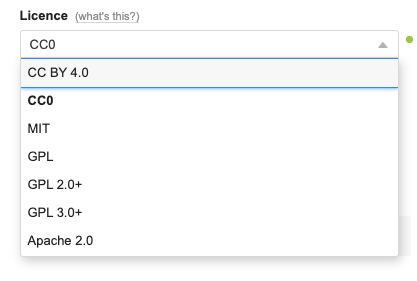
\includegraphics[scale=0.7]{figures/lic.png}}
  \caption{Interface allowing the choice from various licencing options as implemented by the Figshare repository.}
  \label{fig:lic}
\end{figure}

\section{Research repositories}
\label{sec:research}

Data and publication repositories have evolved, at least until recently, as separate platforms; as outlined in the previous section, this was caused in part by the particular features \glspl{ntro} require and, at the same time, by the specific workflows traditional research publishing employs, such as peer review or journal production processes.

Nevertheless, the reproducibility crisis demonstrated the need to have all research outputs available for review at the same time, and having them presented in a consolidated manner can speed up the verification process. From a more technical point of view, this can be accomplished in two manners:
\begin{enumerate}
    \item Develop or employ existing technologies for interlinking research outputs, such as \gls{rdf} or \gls{oai}-\gls{pmh}\footnote{\url{https://www.openarchives.org/pmh/}}.
    \item Aggregate all research outputs on a single repository.
\end{enumerate}

Given the current technology and librarianship space, the first solution is in most cases the most feasible; this is due to the existing infrastructure and the large volume of publications already stored on repositories. To be able to link research outputs in a usable manner, two dimensions need to be considered.

First, researchers need to be able to discern and follow the links; an implementation of this is the mean by which papers and data are frequently linked nowadays. As a result of the new policies around research data sharing, publishers often require authors to upload supporting artefacts to other repositories\cite{elsdat,scidat} and include in articles a statement explaining how they can be accessed; at the same time, the repositories holding \glspl{ntro} can link back to the published article. A full example of this is included in Fig. \ref{fig:link}. This can be facilitated by the use of \glspl{pid}, which, on one hand, distil the linking information in a concise form and, on the other, provide a persistent mean of pointing to the current location of the output, even if the original repository ceased to function and the artefact was transferred elsewhere; this second feature is of utmost importance for physically published media, which is obviously \emph{immutable} and thus, cannot be modified in order to amend links.

\begin{figure}[ht!]
\centering
\begin{subfigure}{0.9\textwidth}
  \fbox{
\includegraphics[width=1\linewidth]{figures/pub.png}}
  \caption{Data accessibility statement linking research article to dataset stored on a specialised repository.}
  \label{subfig:paper2data}
\end{subfigure}
\begin{subfigure}{0.9\textwidth}
  \fbox{
\includegraphics[width=1\linewidth]{figures/dryad.png}}  
  \caption{Reference to the published journal article supported by the dataset which is hosted on the Dryad Digital Repository.}
  \label{subfig:data2paper}
\end{subfigure}
\caption{Bidirectional link between a published journal article and its supporting dataset, source: House et. al. (2020) \emph{Social norms and cultural diversity in the development of third-party punishment}, \texttt{DOI}: 10.1098/rspb.2019.2794.}
\label{fig:link}
\end{figure}

Second, systems that are used to store and disseminate outputs, including but not limited to repositories, need to be able to create, discover and traverse the links between outputs. This is one of the main purposes of the \gls{fair} principles, its importance stemming from the nature of the \gls{www}.

To further emphasise this point, consider the case of \emph{searching} for the study in Fig. \ref{fig:link} using a specialised research search engine. In a naive implementation, such an engine would consider only the metadata of the published paper; this could prove inefficient in cases where the user performs queries pertaining to details of the R\footnote{\url{https://www.r-project.org/}} implementation of the methods used in the study, and which are detailed only in the data package. A search system which is able to understand the link between the paper and the \gls{ntro} could present the user with complete information on the study by providing a consolidated view including both outputs.

Bibliographic metadata is of utmost importance in allowing systems to process links between research outputs. First, metadata needs to include correct and complete information on the artefacts, in order to provide as many opportunities as possible for discovering links between various outputs. Second, as outlined the the \gls{fair} principles, metadata needs to be exposed in a format that promotes interoperability, both at the semantic and syntactic level. Repositories, especially those developed in the early days of the \gls{www}, might struggle with interoperability, as their internal metadata representation did not consider the requirement of allowing other systems to consume it. In Chapter \ref{ch:rdf} a solution for such cases is presented; this solution makes use of \gls{rdf}, this model displaying a series of advantages in terms of linking, as at its core, it implements a knowledge graph.

The second solution to presenting all artefacts pertaining to a research study in the same context revolves around using the same repository for both traditional and non-traditional outputs. In some ways, especially if the distributed nature of the \gls{www} is considered, this can be viewed as counter-intuitive; having each output reside on a platform that best fits its particularities and having them linked as explained above is fully achieving the full potential of the linked \gls{www}.

At the same time, certain realities surrounding the research workflows need to be considered. For example, in a distributed model, researchers might find cumbersome having to upload each output to a different platform, especially if each platform implements the upload process in different manners. In \cite{austin}, the authors note that the amount of time preparing outputs for publishing is a \emph{``major disincentive''} for sharing on repositories, researchers preferring to spend their time on activities which can be credited. Similarly, even in most streamlined linking implementations, consumers of research will still need to follow the various links between outputs and work around the various interfaces repositories employ. Another fact to consider revolves around the administration of repositories; having multiple solutions to maintain can increase the burden on both technology and library resources.

Apart from the consolidation of outputs, using a single repository can provide opportunities for both improving and creating new research workflows. This is best exhibited by the popularisation of new types of outputs, such as:
\begin{itemize}
    \item Pre-registrations: commitment of research plans before executing them, see for example the \emph{``Preregistration Challenge''\footnote{\url{https://osf.io/prereg}}}.
    \item \glspl{dmp}: documents that detail how data will be acquired, managed, analysed and preserved; as these usually describe what repositories will be used,  it seems logical that they are also kept along with the data and other artefacts (for an example see \href{https://doi.org/10.5281/zenodo.1243763}{\texttt{DOI}:10.5281/zenodo.1243763}).
    \item Preprints: while ar$\chi$iv\footnote{\url{https://arxiv.org}}, one of the most well-known \emph{preprint servers} was launched in 1991, preprints came to prominence lately due to their intrinsic property of delivering research results fast, unhindered by traditional publishing practices. For example, during the 2020 \gls{covid} epidemic, over 2000 preprints on the subject have been \emph{posted} on medRxiv\footnote{\url{https://medrxiv.org}} and bioRxiv\footnote{\url{https://biorxiv.org}} between January and April.
\end{itemize}

Three paths to shifting from a specialised repository (e.g., \gls{ir} or data) to a general research repository, able to hold and manage in an meaningful manner any type of research output, can be considered: 
\begin{enumerate}
    \item Develop new features for an existing repository in order to support new types of outputs. For example, Invenio\footnote{\url{https://invenio-software.org/}}, a repository first released in 2002 and developed as an \gls{ir} and library system evolved to be a system which can also hold datasets\cite{invenioabout}, software and other types of outputs, as best demonstrated by ZENODO, which deploys Invenio in its backend. As a reversed route, Figshare, a product that started as a data repository has evolved to also support outputs specific for \glspl{ir}\cite{figntro}.
    \item Migrate existing content to a repository able to manage any kind of outputs. Apart from the opportunity to modernise the repository infrastructure and consolidate administrative, operations or technological resources, this solution might also resolve certain issues generated by commercial, contractual or leadership changes (for an example see the acquisition of Bepress, the developer of the Digital Commons repository\footnote{\url{https://www.bepress.com/products/digital-commons/}}, by Elsevier\cite{bels}). The migration route is further discussed in Chapter \ref{ch:migration}.
    \item Develop distributed repositories: this solution would still consist of multiple systems, each holding various types of outputs, but a single point of entry, for both uploading and consuming content would be provided. In \cite{coar}, the authors make the case for \emph{networked repositories}, in which \emph{}``cross-repository connections are established by introducing bi-directional links as a result of an interaction between resources in different repositories, or by overlay services that consume activity metadata exposed by repositories''. 
\end{enumerate}

While the first two options above are strictly focused on discrete repositories, the third one considers the development of external interoperability frameworks, capable of extracting and providing information from and to the various systems involved in the scholarly workflow. As an example of such infrastructure, Scholix\footnote{\url{https://scholix.org}}, a framework for \emph{``Scholarly Link Exchange''}, currently consists of over 250 million links between research literature and datasets residing in various repositories; any external system can make use of the graph implemented by it in order to present all outputs pertaining to a research study in a consolidated manner. In terms of implementation, Scholix relies on information regarding \emph{associated content} provided by various stakeholders such as repositories, scholarly publishers, or \gls{doi} minting agencies. It is worth noting that the latter can easily become the backbone of such interoperability infrastructure due to the \gls{doi}'s increase in popularity coupled with the requirement for repositories to provide at least minimal metadata for each minted identifier. As such, most agencies provide nowadays the possibility of providing information on known relations between outputs via established relationship types vocabularies\footnote{For an example on how Crossref, a \gls{doi} minting agency, implements this see the \emph{``Relationships between different research objects''} section at \url{https://www.crossref.org/education/content-registration/structural-metadata/\#00040}.}.

Despite the mean of achieving it not being concrete, the vision of research repositories that encompass the plethora of outputs available nowadays is both clear and widely accepted in the community. In \cite{salo}, the author argues that \glspl{ir} should look beyond literature, as otherwise a repository will not fully justify its existence. Even by coming back to the definition in \cite{lynch}, it can be seen that \glspl{ir} were never meant to be limited to certain types of content, mostly peer-reviewed scientific literature, but to cater to any needs the researchers, their workflows and the current societal circumstances call for. Thus, it is important to look at the various options of achieving this vision and let the stakeholders in the scientific endeavour decide which is the best to employ. In the next chapters, original research on certain features that could be implemented in research repositories is presented; the common theme among these is the adaption of techniques specific to software engineering and of technologies employed in other types of applications in the last few decades to the area of digital libraries, touching on all paths presented above, which could lead to a new generation of research repositories.

\newpage

\section{Open Source repositories}
\label{sec:os}

While open science is a relatively new movement, the world of librarianship always took a more \emph{public} approach to the services it delivers, in line with the philosophy that knowledge should be shared freely both across the research community and society as a whole; an interesting effect of this is the development of multiple open source repository solutions.

DSpace\footnote{\url{https://duraspace.org/dspace/}} was first released in 2002 as a solution for the submission, management and preservation of digital records. It features a web interface, a backend written in the Java\footnote{\url{https://www.java.com/}} programming language, a relational database for holding metadata, and a search engine. DSpace uses \gls{dcmt} as its default metadata schema, and includes facilities for \gls{doi} minting, record versioning, and exports via \gls{oai}-\gls{pmh}. DSpace is the most popular repository solution, with almost $2000$ instances recorded on the \gls{roar}\footnote{\url{http://roar.eprints.org/}}.

EPrints\footnote{\url{https://www.eprints.org/}} is considered to be the first digital repository solution, with the initial release in 2000 and with almost 700 instances registered in \gls{roar}. It features both a web and a command line interface and is written in the Perl\footnote{\url{https://www.perl.org/}} programming language. Metadata is stored in a relational database using an internal hierarchical model. The architecture of EPrints is based on \emph{plugins}, which allows customising any functional aspect of the repository.

Fedora\footnote{Not to be confused with the Linux distribution sponsored by Red Hat Inc.} (Flexible Extensible Digital Object Repository Architecture) Commons\footnote{\url{https://duraspace.org/fedora/}} is a digital asset management system which can be used as the foundation of other repositories, from which Samvera\footnote{\url{https://samvera.org/}} (previously known as Hydra) and Islandora\footnote{\url{https://islandora.ca/}} are the most popular. With the first public release dating to 2004, Fedora distinguishes itself by its flexibility, which results from two architectural features. First, it allows seamless conversions from its data model to \gls{rdf}, which enable the usage of any metadata vocabulary for describing bibliographic records and the \emph{linkage} of information residing on external systems; the benefits of \gls{rdf} will be further discussed in Chapter \ref{ch:rdf}. Second, Fedora opts for a service-based design, which allows plugging in any new modules via \gls{rest} \glspl{api}, while ensuring that these conform to the business logic rules of the core system. Fedora is implemented using the Java programming language and uses relational databases for holding metadata records.

Invenio is a software suite which allows running an online, large-scale document repository or digital library. Its features cover all aspects of such repositories, including document ingestion, classification, ranking, indexing, curation and dissemination\cite{kaplun, glauner}; the architecture of the software is highly modular, each component being in charge of one the mentioned aspects or other additional features. Currently, it is being developed by an international developer community and is released as open source software under the second version of \gls{gpl}. The software platform is built using the Python programming language uses a relational database for metadata. Records are represented internally using an \gls{xml} derivative of the MARC 21\footnote{\url{https://www.loc.gov/marc/bibliographic/}} bibliographic format, which is widely used for the representation and exchange of bibliographic, authority, holdings, classification, and community information data in machine-readable form.

While the projects presented up to this point focused mainly on delivering \gls{ir} solutions, Dataverse\footnote{\url{https://dataverse.org/}} is a repository system that treats data as a first-class citizen. Thus, it has aligned its development roadmap with the \gls{fair} principles, including features such as \gls{doi} minting, machine-readable metadata embedded in dataset landing pages, interoperability with external metadata sources, and facilities for licencing and controlling access to datasets. Dataverse also focuses on facilitating and capturing data citations, adhering to the philosphy that \glspl{ntro} can also make an impact in research. Also different from the other reposiroty solutions are the means through with Dataverse can store and present to users complex file formats and non-trivial directory structures. The repository is implemented in the Java programming language and stores metadata in a relational database.

An important aspect shared by all the mentioned repository projects relates to their governance; the development of these solutions is steered by panels of users and experts in the fields of librarianship or information management, in order to ensure that the deliverables are always aligned to the requirements of the research community. For example, at the time of this work, 16 out of the 21 memebers of DSpace's leadership group were affiliated with academic institutions\cite{dspacelead}. Similarly, the Invenio project originated in the world of high-energy physics, being used in production by both the European Organisation for Nuclear Research (CERN) Document Server (CDS), and the INSPIRE repository which is curated by a collaboration of scientist from the Deutsches Elektronen-Synchrotron (DESY), Fermi National Accelerator Laboratory (FNAL), and SLAC National Accelerator Laboratory.

These communities play a crucial role in the development of all repository solutions, not only the open source ones, as they most often define the principles all digital libraries should adhere to. As a result of direct competition, commercial repository vendors must implement the functionalities present in their open source counterparts, this ensuring that the same level of service quality is offered to institutions and researchers that do not possess the technical or administrative resources to deploy a stand-alone repository.

    \chapter{Research dissemination, reuse, and licencing}
        \label{ch:blockchain}
        Chapter \ref{ch:evolution} described the various legal issues surrounding the publishing of research outputs in general and datasets in particular and hinted that repositories can help alleviate these issues by providing technological solutions that can either implement compliance or help users take informed decisions on legal aspects.

In recent years, the rise of \emph{blockchain} technologies such as Bitcoin\footnote{\url{https://bitcoin.org/}} or Ethereum\footnote{\url{https://ethereum.org/}}  has been examined as a potential mean of solving some of these issues, the movement in this direction being fuelled, in part, by the increase in interest due to usage in the financial domain (e.g., Bitcoin). At a very high level, the blockchain allows recording data and verifying its authenticity without the need for a central authority. In the most popular implementations, each participant in a blockchain holds a copy of the whole record set and each record is linked to a previous one by a cryptographic value, distilled using the records' content; thus, even the most trivial change would propagate across the whole chain, signalling the modification. The basic idea behind blockchains can prove useful in areas where authenticity, provenance, and anonymization are important, research being one of them. In \cite{dsbc} the authors have identified a number of ways in which blockchains could be implemented across the scholarly workflow, such as:

\begin{itemize}
    \item Digital rights management: a blockchain system can easily record ownership and ensure that future usage of data respects and attributes  ownership along with any associated stipulations. This could prove useful also in terms of counting citations and understanding how outputs are further reused.
    \item Hypothesis registration: allow researchers to signal a discovery, proof, or new dataset while providing evidence of ownership in any future instance.
    \item Study pre-registration: while becoming a common practice, it can be difficult to ensure that these plans are not modified while the experiments are ongoing, in order to mask potential discrepancies with the actual results; a blockchain systems could easily detect such a change.
    \item Data anonymisation and provenance: this can prove to be of utmost importance for medical and pharmacological research, where, on one hand, stringent requirements on patient privacy and data anonymisation\footnote{Refer to Section \ref{subsec:legal}} are in place, and, on the other hand, the origin of the data should be verifiable. The use of cryptographic controls and the distributed architecture of blockchain systems can help with these challenges.
\end{itemize}

The first point above presents interest, as licencing and distribution is most often closely linked to the perceptions researchers have on sharing outputs. Various studies \cite{federer,kim} have identified \emph{perceived risks} in data sharing activities, largely due to the conditioning of academic success on publication volume and impact. A survey among Wellcome Trust awardees showed that \emph{``the main barriers to data sharing are  the fear for misuse and misinterpretation of data, the fear to lose publication opportunities [\ldots]''} \cite{wellcome}. Another study on articles published in Science between 2011 and 2012 found out that 11\% of the authors refuse to share data if the requester does not provide information on how the material will be further used\cite{stodden}.

A particular blockchain technology, \emph{smart contracts} can approach these issues from a technological angle. They are a a protocol which allows to digitally facilitate, verify, or enforce the negotiation and performance of a contract. Initially introduced in 1996-1997\cite{szabo}, they came back into the spotlight along the other blockchain technologies as a mean of verifying various types of transactions. 

The remaining of the chapter proposes a solution to research output licencing that uses smart contracts and blockchains to record dissemination and reuse actions; from a technology point of view, this solution uses three building blocks.

The first component, the blockchain, is a continuously growing list of records linked using cryptographically calculated values stored in each block. In its most popular implementation, Bitcoin, each block records the \emph{hash} value of the previous block, a timestamp, and data about multiple \emph{transactions} (algorithmic operations with one or more inputs and one or more outputs); such a list of transactions is called a \emph{ledger}. Most such systems are implemented as a peer-to-peer network, in which each node stores a full copy of the blockchain, thus removing the requirement for a central authority that needs to verify all transaction data; practically, such systems implement a distributed database in which consensus is achieved via the proof for validating the sequence of blocks.

Second, Ethereum is an open platform for building decentralized applications on top of blockchains; it defines a number of protocols for running arbitrarily complex algorithms on the network. Such code is ran on Ethereum virtual machines, which are Turing complete; these virtual machines are stored on each node participating in the network, and each issued instruction is ran on every node. A valid state transition on these virtual machines is one which comes through a transaction\cite{gavin}. Ethereum also implements its own value token, called \emph{ether}, but the way in which this is used depends on the application being implemented. One purpose of the value token is to provide a representation of the physical resources required for participating in the network (e.g., electrical power), and, for example, most commonly each operation executed on the virtual machines carries an inherent cost, denoted as \emph{gas}\cite{gavin}.

Last, at the core of the proposed solution stands the implementation of smart contracts in Ethereum. This platform includes two types of \emph{accounts}. \glspl{eoa} sre controlled usually by human actors via private cryptographic keys while contract accounts are controlled by the code to be ran on the virtual machines, which can be activated only by an externally owned account (for a more detailed explanation see \cite{ethdocs}. Contract accounts implement smart contracts, systems that usually contain value tokens that will be unlocked only if certain conditions are met. Solidity is an object-oriented, statically typed, high-level language used for implementing smart contracts on the Ethereum virtual machine\cite{solidity}. A contract in Solidity is defined, similar to a class in traditional object-oriented programming, as a collection of functions and data. The invocations of the functions, as well as a history of the values of the stored data, are stored in the underlying blockchain, making the execution of the smart contract fully traceable.

Using these components the proposed solution for tracking digital rights enforcement over research outputs can be be built; for clarity we will assume the the shared research output is a dataset. First, the two types of accounts required by the Ethereum network need to be defined; there will be two externally \glspl{eoa}, one for the author that initially publishes the dataset, and one for the entity the wishes to reuse it. The contract account is associated to the smart contract code that will regulate reuse.

In terms of stored data, the following entities are considered:
\begin{enumerate}
\item Author account address: this variable simply records the address of the \gls{eoa} of the author (or producer) of the output.
\item Dataset hash: this is a cryptographic hash of the research dataset that is to be published. Note that the smart
contract (and underlying infrastructure) does not store the actual data files, but only their hash; the complete content can continue to reside
on the standard repository infrastructure.
\item Dataset terms hash: this is a cryptographic hash of the terms and conditions, specifying the way in which
the published dataset might be reused. The same approach as with the dataset, of not storing the actual contents of the terms, is taken, as repositories most often have specific means of handling the application of licencing (see Fig. \ref{fig:lic}). Nevertheless, in some cases the author might opt for using a custom definition of the terms (e.g., embargoes such as \emph{``reusers should not publish journal articles on findings based on the original dataset for one year since the initial release of the data''}) which cannot be hosted by such platforms, or there simply might be a requirement to ensure the preservation of the terms and, in such cases, the full text could be stored on the blockchain by compressing it\cite{brown}.
\item Data reuser account address: similar to the first item in this list, this variable records the \gls{eoa} address of the entity planning on reusing the data set.
\item Reuse work hash: this variable records a hash (or any other type of appropriate information, such as a \gls{doi}) for the work that reuses the original data set. This will ensure that the complete cycle of reuse is recorded on the blockchain, making it easy to inspect at any future moment.
\end{enumerate}

The smart contract will consist of three functions that need to be called in the following order:
\begin{enumerate}
\item Publish dataset: this function will record the author account address, dataset hash and dataset terms hash variables; optionally, it can emit an event (see the \emph{Events} section of \cite{solidity}) in order to advertise the release of the dataset and enable certain automatic workflows (e.g., a system similar to a \gls{rss} feed could be put in place to monitor the release of new data).
\item Release dataset: this function records the data reuser account address, conceptually stating that the author of the dataset released it under specific terms to the requesting entity.
\item Publish \emph{rework}: this function records the reuse work hash, storing information about how the dataset has been reused, and closing the execution of the contract.
\end{enumerate}

These three functions describe how the smart contract should be developed and executed from a practical point of view, integrated with the current research workflows. As soon as a dataset is published, a version of the smart contract should be deployed and the first function should be called in order to record the terms under which the work can be reused. When there is a wish to access the dataset, the two parties (author and reuser) should come to an agreement on following these terms and record this on the blockchain by using the second function. The proof that the terms were actually followed will be recorded by calling the last function. A discussion on this last step relates to the entity that should call this operation; here it is considered that the reuser can do this, testifying that the established terms have been followed, and recording this in the permanent record of the blockchain. If this is deemed insufficient, an additional step can be added, in which the original author of the dataset, or any other suitable entity, verifies that terms were indeed obeyed, closing the execution of the contract.

An implementation of the smart contract conceptually described above, using the Solidity language, is included in Fig. \ref{lst:solidity}.

\begin{figure}
\lstinputlisting[language=C,
                 frame=tblr,
                 captionpos=b,
                 showspaces=false,
                 showstringspaces=false,
                 showtabs=false,
                 stepnumber=2,
                 numbersep=4pt,
                 basicstyle=\fontsize{8}{7}\ttfamily]
  {figures/publish.txt}
  \caption{Solidity smart contract implementing the research data reuse terms management workflow.}
  \label{lst:solidity}
\end{figure}

Two minor implementations details can be observed:
\begin{itemize}
\item The \texttt{requestDataset} function allows expressing the intent to access the published dataset. This
is implemented in order to further automate the workflow, as without this functionality the requester would have to contact the author of the dataset using some other channel, such as email or
the features provided by the repository.
\item Events are implemented and emitted at each invocation of the functions of the smart contract; as mentioned, this could
prove useful for automating certain external workflows building upon the smart contract.
\end{itemize}

A brief analysis of the costs of running such a routine on the Ethereum Virtual Machine and network is presented below. This was carried out by considering the gas requirement for a full invocation of the smart contract; this comprises of two elements\footnote{Both concepts are explained in depth in Section \emph{Account Types, Gas, and Transactions} of \cite{ethdocs}}:

\begin{itemize}
    \item The transaction cost of the functions in the smart contract (the gas cost for setting up the functions on the blockchain).
    \item The actual execution cost; this depends on how much processing steps are required by an Ethereum Virtual Machine for executing the functions.
\end{itemize}

The costs are expressed in Ethereum network gas; a
rate of $2*10^{-9}$ ether per gas used was set, with the price of 180.66 US dollars per ether (value for April 2020). The results are presented in Table \ref{tbl:eth}. 
\begin{table}
\begin{tabular}{ |c|c|c|c|c| } 
 \hline
 Operation name & Transaction cost & Execution cost & Total gas & USD price \\
 \hline
 \hline
 Creating contract & 613654 & 421050 & 1034704 & \$0.93123 \\
 \hline
 publishDataset & 55140 & 33612 & 88752 & \$0.07988 \\
 \hline
 requestDataset & 23313 & 1913 & 25226 & \$0.0227 \\
 \hline
 releaseDataset & 44728 & 23456 & 68184 & \$0.06136 \\
 \hline
 publishRework & 30134 & 8734 & 38868 & \$0.03497 \\
 \hline
\end{tabular}
\caption{Gas costs as defined by the Ethereum Virtual Machine and network of the implemented smart contract for rights management of research data. Equivalents in US dollars, calculated using the rates available in April 2020, are included. While the \emph{transaction cost} is an estimation of work required to define the contract on the network, the \emph{execution cost} considers the actual execution cost of the transaction, based on the number of computing operations.}
\label{tbl:eth}
\end{table}

As it can be observed, the total cost for setting up and executing the contract is below two US dollars. If researchers would be to support these costs, as opposed to having the
network fully sustained by research publishers or any other scholarly communication entity, they are still negligible when compared to other usual expenses, such as, for example, \glspl{apc} or \gls{oa} publishing: the costs required by Springer Nature and Elsevier can easily go in the range of thousands of US dollars\cite{elsevierapc,snoa}. 

An interesting aspect that stems from this analysis and takes inspiration from the widespread use of blockchain technologies in financial workflows relates to the implementation of incentives for both publishing research data and also considering replication studies. Given that the framework for implementing such mechanisms is inherent in the targeted platform, it is fairly easy to extend the smart contract to consider, for example, awarding a number of value tokens (ethers) when a new data set is published; similarly, a number of value tokens could be subtracted from the \gls{eoa} of the reuser, thus creating further incentives to stay in line with the established terms.

    \chapter{Linked data in research repositories}
        \label{ch:rdf}
        \subsection{Current implementation}
\label{sec:curr}

Currently, figshare holds all its metadata in a relational database \cite{figsupport}, with
tables for each of the entities required for describing a record. The reasoning behind
this choice includes the team's experience with relational systems, the extensive commercial
support for such solutions, and the high availability and clustering options provided by
these systems even before figshare's inception.

While the current system continues to function well, certain shortcomings were observed
when it came to implementing a number of features requested by figshare's users and customers; the two main requests that triggered the idea of using an RDF-based model are:

\begin{enumerate}
\item Provide the ability to export metadata in various formats, both predefined in the system and defined ad hoc by end users. Currently, figshare allows exporting metadata in a fixed set of
formats, both in its OAI-PMH interface and web application (see Fig. \ref{fig:figexport}), but this is
lacking in both number of formats and the actual metadata which is available when exporting (e.g., almost all options do not contain information about the files pertaining to a record).

\begin{figure}[thpb]
  \centering
  % fbox will add a border around the figure
  \fbox{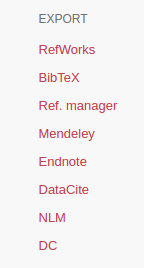
\includegraphics[scale=0.5]{figures/figshare_export.png}}
  \caption{Formats exposed by figshare for exporting bibliographical information via its web interface.}
  \label{fig:figexport}
\end{figure}

\item Provide an easy mechanism for enhancing the main metadata set. Currently figshare allows
institutional customers to define so-called \emph{custom metadata fields}, which extend the 
main set to include information such as, but not limited to, geographical
location information, retention dates, or archival markers; the interface for defining such fields
is presented in Fig. \ref{fig:caf}. The main limitation of these fields is that they currently
cannot be exported in any standard metadata format (e.g., via OAI-PMH) due to their lack of a
proper \emph{definition}; for example, when defining a field for holding geographical location
information, there is no mean of mentioning that this field follows the definition of the Dublin
Core Metadata Terms \emph{spatial} one (URI: \nolinkurl{http://dublincore.org/documents/dcmi-terms/#terms-spatial}). This limitation is not only one of the user interface, but also of the application's data model, as the relational scheme is not easy to modify in order to accommodate all the possible definitions and configurations.

\begin{figure}[thpb]
  \centering
  % fbox will add a border around the figure
  \fbox{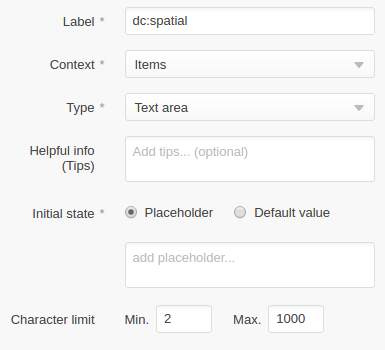
\includegraphics[scale=0.4]{figures/field.png}}
  \caption{Figshare interface that allows institutional clients to define custom metadata fields that can be filled in when creating a new record. Options for defining the type of the value (plain string, date field, etc.), certain validations, and guiding information are included.}
  \label{fig:caf}
\end{figure}

\end{enumerate}

While exploring possible solutions to the issues above it became clear that implementing an RDF-based model and workflows would be beneficial not only for answering the two requirements, but also for creating an extensible system upon which various use-cases can build upon. The solution is described in the next subsection.


\subsection{Towards an RDF model}
\label{sec:rdf}

The first challenge we need to overcome in building an RDF model is mapping all of figshare's metadata fields, defined as columns in the relational model, to a well-defined ontology, vocabulary of terms; this is required in order to
be able to properly identify the elements of the triples, as previously explained. In order to achieve this, we can either provide our own definition for each attribute in the relational model and then publish the whole set along with the RDF graph, or use an established vocabulary. We chose the second option, in order to comply with figshare's stated mission to use well-known standards, and avoid the \emph{not invented here} fallacy; moreover, this approach has already been explored by the figmeta project \cite{figmeta}, and this would speed up the development of our end-to-end solution.

Figmeta employs the VIVO Core Ontology \cite{vivo}. For each column in the relational model, the field in the ontology which is the closest to figshare's internal
\emph{definition} of the column's contents was chosen; it is worth noting that finding an objective measure of how well this mapping was done is quite difficult as figshare never provided an
exact meaning for each of the columns in the relational model (or metadata fields it expects its records to have). Having this ontology, triples describing a figshare item can be built,
and these can be visualized in a graph such as the one in Fig. \ref{fig:graph}.

\begin{figure*}[thpb]
  \centering
  % fbox will add a border around the figure
  \fbox{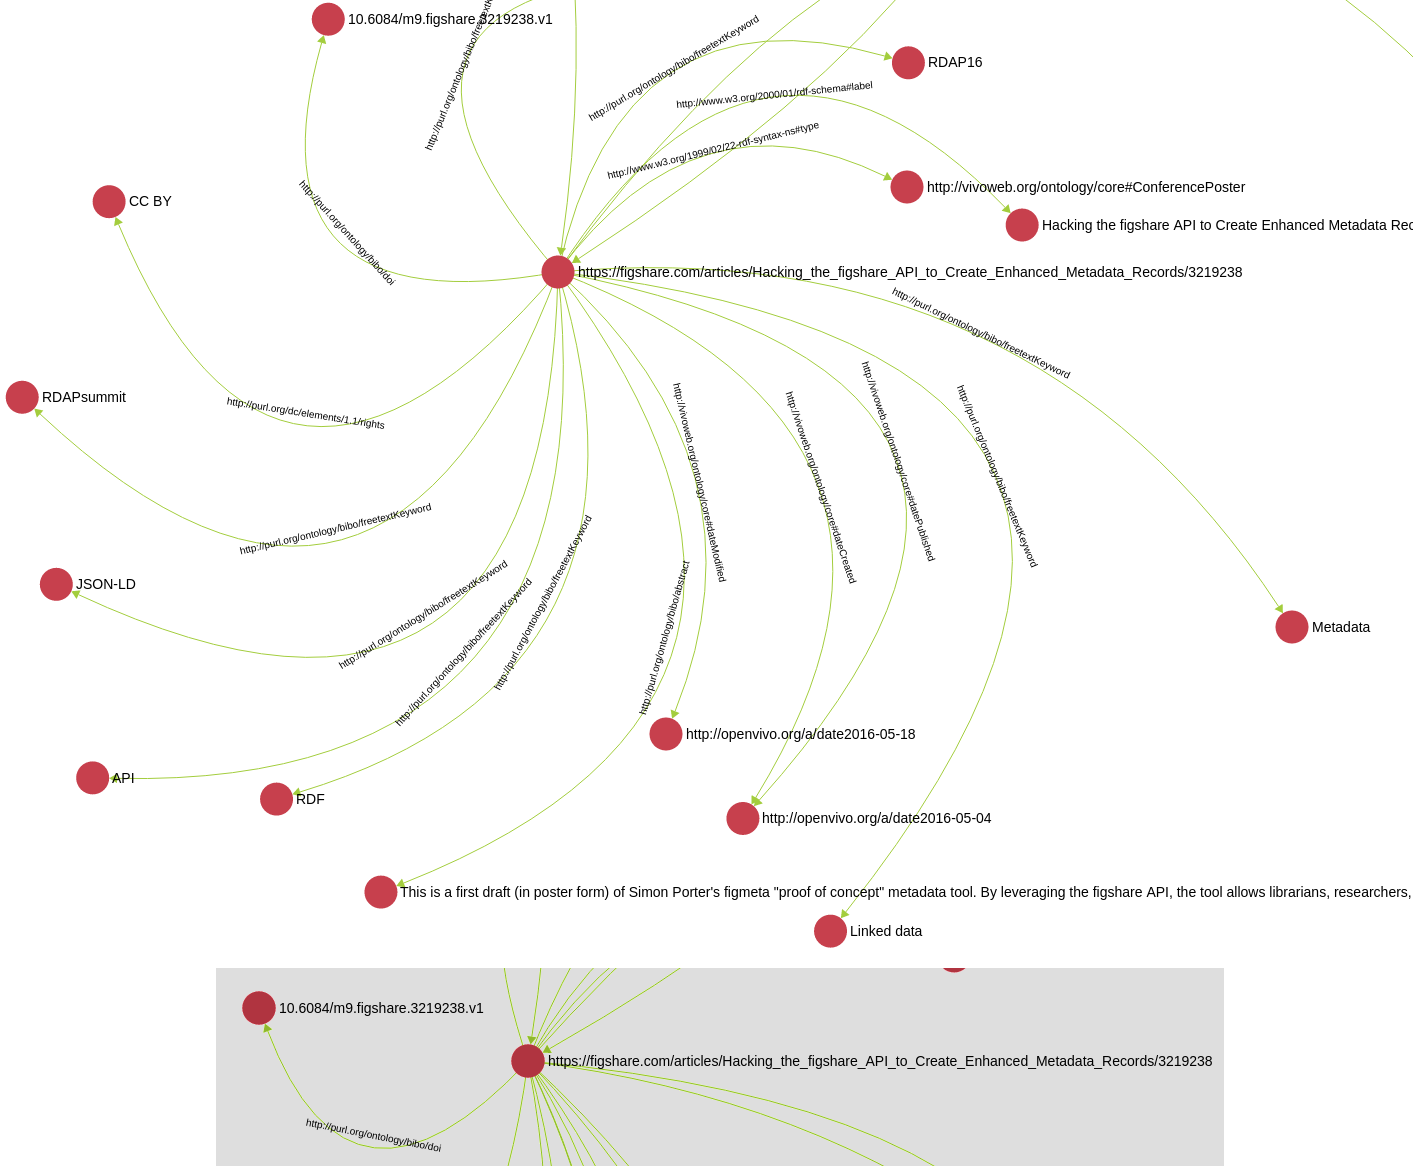
\includegraphics[scale=0.35]{figures/rdf.png}}
  \caption{A figshare item's RDF graph visualized. Vertices are subjects or objects, while edges are the predicates; edges are always directed from subject to object. The lower snapshot details one of the triples; the predicate is  from the BIBO ontology \cite{bibo}, used by VIVO, and associates the subject (a research record) with a Digital Object Identifier (DOI).}
  \label{fig:graph}
\end{figure*}

It is worth noting that this representation is already publicly available in the OAI-PMH interface, under
the RDF \emph{format}.

Our second challenge relates to the definition of custom, user-defined metadata. Here, we distance
from the approach taken by figmeta, which saved additional fields in a JSON-LD (a JavaScript Object Notation serialization of RDF triples) data file of the
record, by implementing an approach which embeds custom defined metadata in the original record
model. In order to achieve this, when defining a custom field, apart from the information
presented in Fig. \ref{fig:caf}, we also request the user to specify the ontology where the field
is defined (e.g., Dublin Core Metadata Terms), and its name in this ontology (e.g., \emph{spatial}).
This makes it very easy to include this new piece of information in the RDF graph; the predicate
becomes the term name and its ontology (e.g., \nolinkurl{http://dublincore.org/documents/dcmi-terms/#spatial}),
and the object the actual value, specified when the record is created. The subject, in the
current configuration, is always the figshare item, but due to the flexibility of the RDF model
it could become any other vertex in the graph (e.g., the file, or the author identifier).

Apart from the flexibility, this approach also has the advantage that it considers all metadata
to be equal. In the current relational model, where table structure cannot change so often, the
core metadata set, which was defined by figshare, is treated as a first-class citizen, while user
defined metadata is lacking certain features; for example, figshare's search system cannot fully search by the custom medatada fields (e.g., retrieve all records for which the \emph{spatial} field has the value ``Appalachian Mountains'', see the figshare search documentation at \cite{figsearch}). Our aim is to have a uniform representation, where all fields require equal effort in terms of development when a certain functionality is considered.

The third challenge we considered relates to the methods used for exporting metadata outside the figshare system. In the current model, this is done by implementing interfaces between the various aspects of the platform (OAI-PMH, web interface, RESTful API) and the relational model; this can become cumbersome, because for each new export format development time needs to be spent in order to provide it, and, even more important, users cannot define
their own preferred output.

RDF graphs can be serialized in various forms, such as the already mentioned JSON-LD, Turtle or N-Triples; the most popular one, nevertheless, is RDF/XML, which leverages the adoption of the XML format and its ecosystem. As most of the formats currently expected by figshare's users are
XML-based, we focused on this format, and noticed that starting from a RDF/XML serialization of our
graph we could easily pivot to any other format by employing Extensile Language Stylesheet Transformations (XSLT), a method for transforming XML documents to other XML representations.

Thus, for example, in order to get a Dublin Core Metadata Terms representation of a record modelled using RDF, two steps need to be performed:
\begin{enumerate}
\item Distil a RDF/XML serialization of the graph. Most RDF tools nowadays already include the means for this transformation, and thus, the development effort for this can be delegated to them.
\item Perform an XSL transformation from the RDF/XML document to the Dublin Core Metadata Terms one; in order to do this a stylesheet as the one in Fig. \ref{lst:xslt} can be employed. Tools for performing the actual transformation are also wide-spread.

\begin{figure*}[!ht]
\lstinputlisting[language=XML,
                 frame=tblr,
                 captionpos=b,
                 showspaces=false,
                 showstringspaces=false,
                 showtabs=false,
                 stepnumber=2,
                 numbersep=4pt,
                 basicstyle=\small]
  {figures/xslt.xml}
  \caption{Example XSL transformation for converting a RDF/XML document to Dublin Core Metadata Terms XML one.}
  \label{lst:xslt}
\end{figure*}
\end{enumerate}

An important advantage of this approach is that, starting from the XML/RDF serialization we provide, users can define their own transformations. This offloads the development work and
provides greater flexibility in terms of metadata output. The system also provides a solid
base for developing other internal features; for example, Fig. \ref{fig:tind_search} presents the way in which the Invenio digital library platform \cite{invenio} can output search results in the Metadata Object Description Schema (MODS) format; as this is also
an XML-based format, implementing the same functionality could be easily achieved via XSL transformations applied to RDF/XML.

\begin{figure*}[t]
  \centering
  % fbox will add a border around the figure
  \fbox{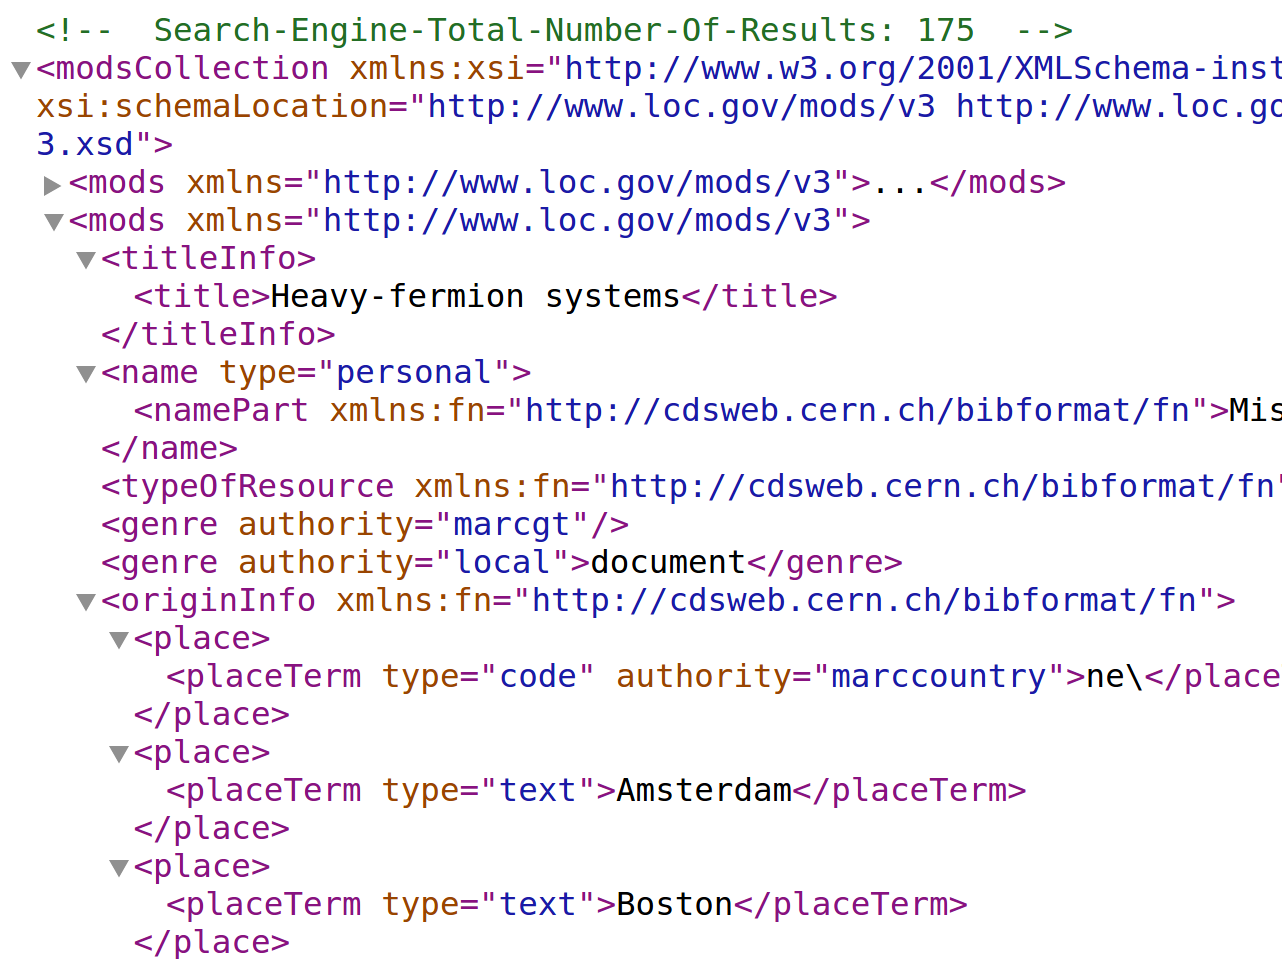
\includegraphics[scale=0.311]{figures/tind.png}}
  \caption{Search results in MODS format as returned by the California Institute of Technology Library Catalog \cite{caltech}, a solution using the Invenio framework.}
  \label{fig:tind_search}
\end{figure*}

Nevertheless, our system does not need to be limited to the RDF/XML representation; JSON-LD becomes more popular nowadays, especially because the predominance of the JSON format across web
applications, and RDF in Attributes (RDFa) starts being used by search engines for
achieving a better understanding of the indexed web pages \cite{googleld}.

%While a full implementation of the described system is not fully available, we provide a proof-of-concept one \cite{poc} which implements the uses-cases previously described and helped us understand the feasibility of the proposal and the ways in which we should proceed with the production-ready system. It is worth noting that for implementing the required operations we leveraged the RDFlib \cite{rdflib} and lxml \cite{lxml} Python libraries. 

After careful consideration, we reached the conclusion that completely replacing the relational model with the RDF one is not desirable, as, for example, we run the risk of loosing important business logic aspects. Instead, the two models can run in parallel, with the RDF one augmenting the current system. This, of course, will provide new challenges, such as maintaining the two sources of truth in sync while not limiting or hindering the operation of neither of them.

    \chapter{Research repository migrations}
        \label{ch:migration}
        As discussed in Section \ref{sec:research} one of the possible paths for pivoting from pure publications or data repositories to research repositories consists of migrating records to a different system. Such a venture needs to be properly planned and executed in order to ensure, on one hand, that no records are lost or corrupted and, on the other hand, that minimal or no downtime is generated. Ideally, migrations would also be an opportunity to curate and enrich the existing corpus by consolidating and correcting bibliographic records. What differentiates such transfers from other data migrations is the required domain knowledge, the particularities of the target and source repositories in the context of the scholarly communications ecosystem, and the structure of the migration package, which includes, among others, bibliographic metadata, record files and usage data.

In this chapter a workflow and technical framework for performing repository migrations is discussed, based on the experience of six such transfers performed between 2018 and 2019. These considered records stored on various repository solutions (DSpace, Bepress Digital Commons\footnote{\url{https://www.bepress.com/products/digital-commons/}}, custom in-house built systems) that had to be moved to the Figshare \gls{saas} repository platform. For this purpose, SLAM (Stateful  Library  Analysis  and  Migration), an \gls{etl} system was developed and successfully employed in order to migrate over $80.000$ records. 

In early 2018 Figshare has started considering the suitability of its repository platform for storing, along with non-traditional research outputs (datasets or scientific software), content which is usually specific to \emph{institutional} repositories (journal articles, theses, monographs)\cite{fir}. While feature-wise this was validated by its hosted preprint servers\cite{chem}, a new challenge was posed, as clients choosing to use Figshare as an institutional repository also had to transfer all content from their existing systems.

Thus, in the first half of 2018, a first migration was performed, transferring records from a Bepress Digital Commons repository. From a technical point of view, a simple Python\footnote{\url{https://www.python.org/}} script was developed for this migration; this script parsed a \gls{csv} report produced by Digital Commons\cite{bepressdash} which contained all metadata and links to the record files\footnote{For records under embargo the files were transferred using a backchannel.}. Using this information, records were created on the Figshare repository using its \gls{api}\footnote{\url{https://api.figshare.com}}. While this migration succeeded, the \emph{naive} technical solution presented a number of issues:
\begin{itemize}
    \item Difficulties with the metadata crosswalk: while a crosswalk was initially set up, mostly based on the definition of the fields in the source and target repositories' schema\footnote{Both DC and Figshare use in-house custom metadata schemas which better fit their business and data model.}, issues were discovered while migrating the records, mainly due to inconsistencies in the values of the fields across the corpus. These issues were fixed on a case-by-case basis, in order to ensure a lossless migration, but it would have been preferred to surface them in the early phases, in order to have the migration script able to mitigate any issues in the final run.
    \item Difficulties in running the migration procedure multiple times: the migration script followed mostly an \emph{all or nothing} approach, where, at each run, it fully migrated all records between repositories. This was discovered to not be desirable, as there was a need to run the script only for those records that failed to migrate (due, for example, to metadata crosswalk issues). After the full migration was completed, there was also a need to apply only some minor corrections to records, without following the full procedure; this was not possible, due to the fact that the script would recreate all records to migrate from scratch on the target repository, as it did not have any \emph{memory} of previous runs\footnote{This issue was amplified by the fact that in the source repository records did not have any type of persistent identifier attached.}. Thus, additional scripts, which only performed the corrections, had to be developed.
    \item The migrations procedure required constant operator supervision: like most migrations, this instance considered a large number of records (over $10.000$) and, ideally, the migration procedure would run with minimal supervision required from operators. While the initial script partially accomplished this, needs for better fault-tolerance and enhanced logging were identified.
\end{itemize}

Given that a number of five other migrations were to be completed between October 2018 and December 2019, and the lessons learned from the initial attempt, it was required to develop a more robust alternative to the naive migration script; this alternative had to adhere to three main design principles:
\begin{enumerate}
    \item Reusability: the system should be usable for multiple migrations without extensive additions or modifications. Thus, it should be able to adapt to the workflows of multiple repositories, metadata schemas, and other concerns specific to each migration.
    \item Statefulness/ idempotence: the system should be able to perform the same migration multiple times, without creating duplicate records on the target repository, and allowing for incremental record improvements with each run. Apart from allowing for corrections to be applied post-migration, this would also support the prototyping phase, where multiple test migrations are performed in order to validate the metadata crosswalks, to verify that no information is lost, and other general workflow aspects.
    \item Fault tolerance: the system should implement fault tolerance mechanisms at all levels, allowing to run migrations of large corpora with minimal supervision, and, at the same time, implement sufficient logging and exception handling to allow operators to identify and correct potential issues.
\end{enumerate}

A number of repository migrations are present in the literature. In \cite{tragedy} the authors describe the process of moving from a DSpace to a Samvera\footnote{\url{https://samvera.org/}} system, while in \cite{challenges} the records were migrated from a solution developed in-house to DSpace. Both instances offer valuable insight into the challenges posed by digital library migrations, especially at the level of bibliographic metadata; on the other hand, both works are focused mostly on a specific use-case and do not propose general technical solutions for other migrations. It is interesting to note that the migration presented by \cite{tragedy} required $2.5$ years of work, while SLAM was employed to carry 5 migrations in 14 months.

The Bridge2Hyku toolkit\cite{bridge} is a collection of tools, including a module for the Hyku repository solution\footnote{\url{https://hyku.samvera.org/}}, aimed at facilitating the import of records into digital libraries based on this software. Similar to SLAM, it includes an analysis component, useful for surfacing and correcting potential metadata issues during the migration. SLAM provides two major improvements over this solution, namely it defines a generic architecture that can be used for migrating records between any two repositories, while also defining a procedural migration workflow in order to create a robust, fault-tolerant and extensible solution.

Following the design principles mentioned previously, SLAM's architecture was devised as presented in Fig. \ref{fig:workflow}; as it is an \gls{etl} system, the easiest way of understanding its operation is by examining the data flow.

\begin{sidewaysfigure}[ht!]
  \centering
  \fbox{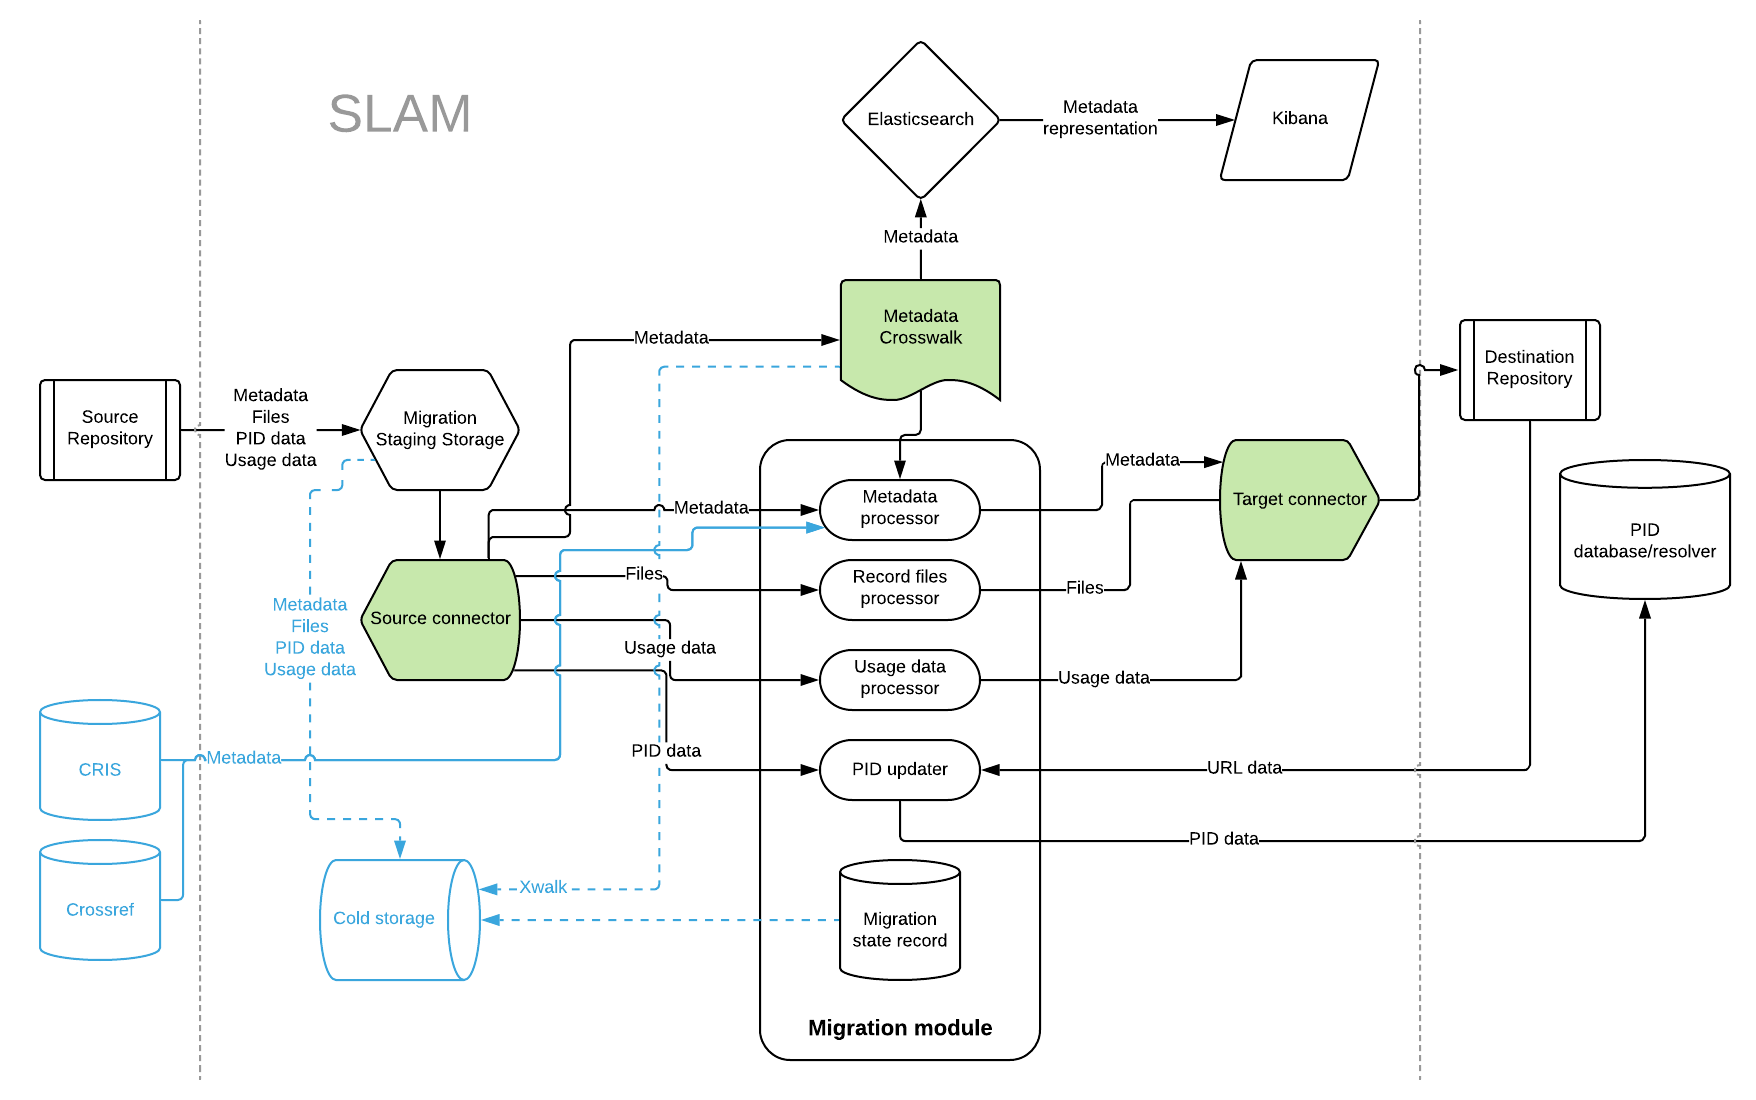
\includegraphics[scale=0.68]{figures/flow.png}}
  \caption{Main components and data flow in SLAM. The system splits the data to be migrated in four logical slices: bibliographic metadata, record files (e.g., \gls{pdf} journal articles), persistent identifiers of records, and usage data (views and downloads). A crosswalk is defined for the metadata and analysed using an Elasticsearch based setup in order to identify potential inconsistencies. The current state of the migration is recorded in a special file, in order to allow for multiple idempotent runs. Metadata can be enriched using external sources, such as a \gls{cris}, or open registries such as Crossref. All migration data is preserved for future reference. Areas in light blue are currently under development. The components highlighted in green need to be adapted for each migration.}
  \label{fig:workflow}
\end{sidewaysfigure}
\afterpage{\clearpage}

The first step concerns extracting all the required information from the source repository. This could be achieved in multiple ways, such as harvesting through an \gls{oai}-\gls{pmh} endpoint or other types of \glspl{api}, using the bulk export functionality implemented by most repository systems, or even by crawling the \gls{html} markup describing records, similar to how search engines do in order to discover web pages. Once this mechanism has been established, practical experience proved that it is beneficial to move this raw data \emph{closer} to the destination repository (to a \emph{staging} area as depicted in Fig. \ref{fig:workflow}). While this transfer might prove cumbersome, especially for large corpora, the operation is required only once. Moreover, having the data close to the destination repository allows faster prototyping and testing of the migration procedure, as network latency and throughput are improved\footnote{This assumes that SLAM is also deployed close to the target repository and the staging storage.}, while also ensuring that the source repository's functioning is not affected in any manner.

Metadata is the first considered aspect; from the migration's point of view, two dimensions are considered, the syntax and the semantics. As discussed in previous chapters, metadata comes in various formats, such as \gls{csv} or \gls{xml} files, and most of these can be easily parsed by openly available software solutions. Of more interest are the semantics of metadata, which stem from the employed \emph{schemas}, such as \gls{dcmt} or DataCite. A schema crosswalk which describes how the fields in the target repository schema should be populated using the source data needs to be set up when transferring records. While this should not be a concern if the two repositories use the same schema, for the performed migrations this was not the case; other reasons for setting up such a crosswalk include:
\begin{enumerate}
    \item Loosely defined schema in at least one of the repositories: certain repository systems do no specify a schema with clear field definitions, validations or applicability. By having the source repository administrators help with setting up a crosswalk, the migration team can avoid issues caused by incomplete understanding of the metadata.
    \item Support the review of the bibliographic records: migrations can prove to be an opportunity for reviewing and amending the records' metadata; for example, infrequently used fields can be completely removed and values which tend to confuse end-users can be moved to other fields.
    \item Ensure that a record on how the migration was performed, from the metadata point of view, is maintained. The crosswalk is considered an output of the migration and is preserved for future reference. 
\end{enumerate}

The crosswalk is tested using Elasticsearch, \emph{``an open source search and analytics engine for all types of data, including textual, numerical, geospatial, structured, and unstructured''}\cite{elastic}. The setup uses the crosswalk to create Elasticsearch \emph{documents} which include all fields as they would be transferred to the destination repository. A Kibana dashboard\footnote{\url{https://www.elastic.co/products/kibana}} is then used to both visually inspect the records and also to enable structured searches across the corpus. This can allow, for example, discovering fields which do not follow a consistent pattern for the values, as the example in Fig. \ref{fig:kibana}. As the crosswalk includes, apart from the field mapping, altering operations that can be performed on each field (e.g., using a standard format for all dates), this analysis can facilitate the review process described by the second point above. While performing actual migrations, a number of inconsistencies about which the source repository administrators were unaware of have been surfaced by SLAM and corrected in the target repository; this is common-place especially in large corpora spanning multiple decades, where the repository metadata workflows and schemas might have changed multiple times.

\begin{figure}[ht!]
  \centering
  \fbox{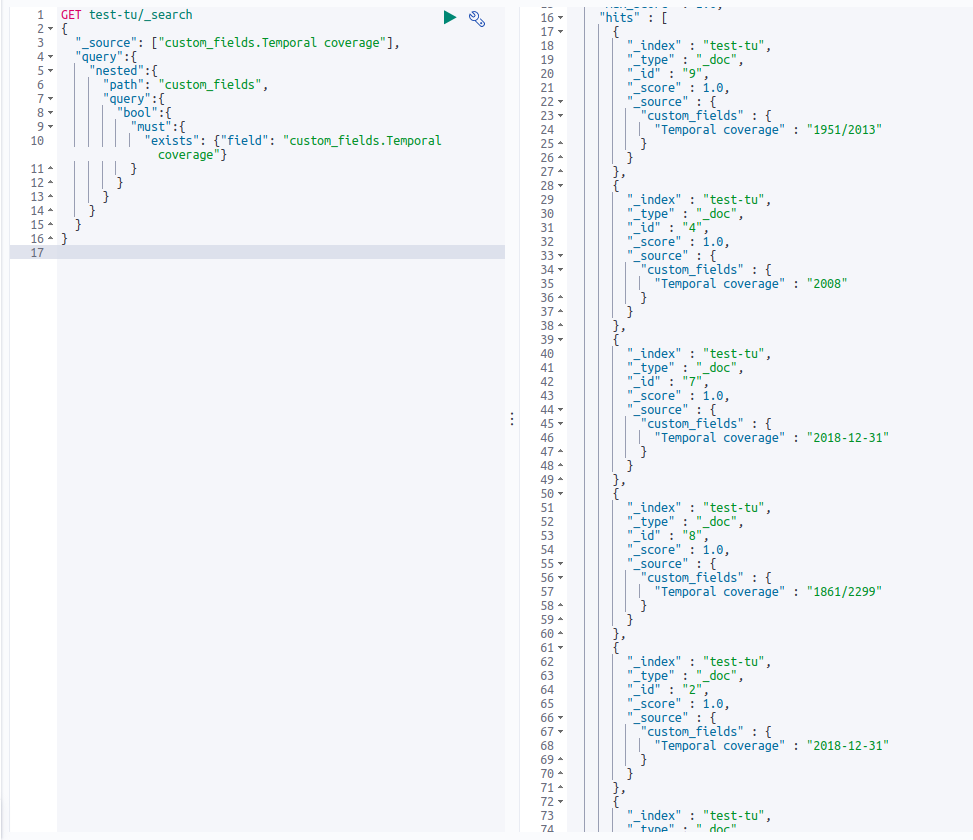
\includegraphics[scale=0.43]{figures/temporal.png}}
  \caption{A view examining the possible values of the temporal coverage field from the Dublin Core schema in a migrated institutional repository corpus. This shows variation in the format of the values (full date, year-only) which can cause issues if migrated to a schema which applies strict validation on date/time values and thus need to be handled by the migration harness. This view is generated using Kibana from the Elasticsearch stack, employed by SLAM for metadata analysis purposes.} 
  \label{fig:kibana}
\end{figure}

Two points should be noted about this component:
\begin{itemize}
    \item This is the only component of the architecture for which an actual implementation is mentioned, namely Elasticsearch. While other solutions could have been chosen, such as the ones included in the Bridge2Hyku toolkit\cite{bridge} (e.g., OpenRefine\footnote{\url{http://openrefine.org/}}), Elasticsearch proved to be the best fit for a highly automated system which requires analysis capabilities; it is a production-grade solution which can index high number of documents and support complex queries, while also providing user-friendly analytical views via Kibana.
    \item Arguments for loading the metadata in the analysis component \emph{without} having it processed through the crosswalk can be brought; such a workflow could provide further insights into various issues of the corpus which are possibly obscured by the crosswalk. The practical experiences of this project did not uncover any such issues, while this specific implementation provided a mean to test the crosswalk, a major migration component; nevertheless, the possibility of having all the raw metadata loaded into an analysis tool before performing any mutation on it needs to be considered for other migrations. It is worth noting that in such cases Elasticsearch might not be the best fit, as due to its architecture it requires a \emph{mapping} in order to load and index documents\cite{mapping}; other solutions, such as Athena\footnote{\url{https://aws.amazon.com/athena/}} could replace it for the analysis component of SLAM.
\end{itemize}

With the crosswalk set up, the migration module can be completed. From a logical point of view, it comprises of four components:
\begin{enumerate}
    \item Metadata processing: this component uses the crosswalk in order to transfer the metadata to the target repository.
    \item File upload: this simply uploads all files associated to a bibliographic record to their new location.
    \item Usage data transfer: most repositories nowadays implement counters for views and downloads of records, and this information, if available, is also transferred to the target repository.
    \item Persistent identifier update: if the records were using \glspl{pid}, such as \glspl{doi}, these are updated to \emph{resolve} to the new locations on the target repository. While the usage of \glspl{pid} is desirable, even across the migrations performed by using SLAM a number of cases where persistent identifiers were not employed were encountered; records were accessible only via \glspl{uri} and these cannot always be transferred between repositories, as each software usually uses its own schema. As this poses an issue for the continuity and preservation of records, implementing identifiers is highly advised before performing a repository migration.
\end{enumerate}

One of the architectural goals of SLAM is idempotence and this is implemented at migration's module level, which is designed as a state machine. A trivial example of such a state machine is included in Fig. \ref{fig:state}. The state machine status is serialised in a persistent database (the current implementation uses a \gls{json} format for state serialisation), each migration run deserialising it in order to determine which operations still need to be applied for each record. Maintaining such a registry provides a number of other benefits:
\begin{itemize}
    \item Facilitates testing and prototyping: this was the original reason behind the architecture, useful especially before the metadata analysis functionality was implemented. If one of the operations required for transferring a record fails, subsequent runs will not require to apply all steps, but only the ones that did not complete. As for each record a separate state section is maintained\footnote{Practical experiences proved that the best way of identifying records is by their unique identifier in the source repository, especially when no universal persistent identifiers are present.}, this becomes especially useful when migrating multiple entries; records which failed to migrate can be easily isolated and subsequently reprocessed.
    \item Allows creating reports on the migration; these are used, for example, to validate that all records were indeed transferred to the target repository.
    \item The migration module becomes portable; as long as the state machine serialisation is accessible, the module can run from different systems and at different points in time.
\end{itemize}

\begin{figure}[ht!]
  \centering
  \fbox{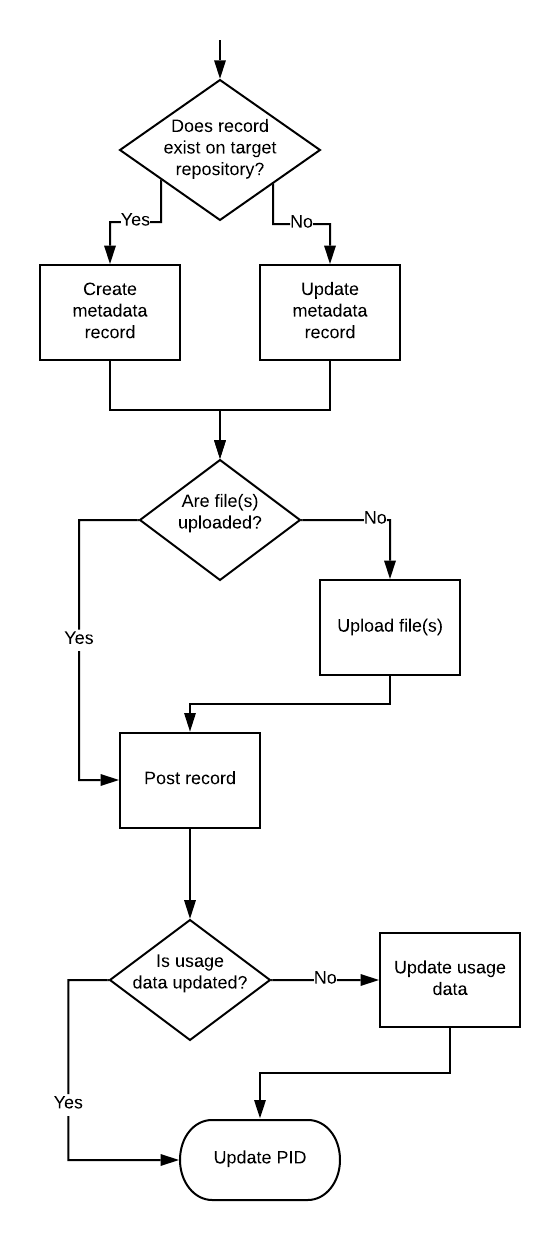
\includegraphics[scale=0.7]{figures/state.png}}
  \caption{A simplified process diagram for migrating a record. Each successful operation is recorded in a persistent database which is used in subsequent runs for deciding the workflow path. For example, files will not be uploaded each time the migration script is ran, thus avoiding duplication.} 
  \label{fig:state}
\end{figure}

The first architectural principle previously presented relates to the reusability of SLAM across migrations. The most common cause of divergence between migrations is related to the differences between repository solutions; SLAM isolates this concern by using two \emph{connectors}, one for the source and one for the target repository. These connectors translate the information to be migrated to and from SLAM's internal data model. Thus, the source connector needs to be able to traverse the staging storage and provide SLAM with all the required record information, while the target connector will upload the records to the new repository (using an \gls{http}-accessible \gls{api} for example). This means that for each migration only 3 parts of SLAM need to be adapted (green highlights in Fig. \ref{fig:workflow}): the source and target connectors, and the metadata crosswalk. All other components can remain unchanged, thus reducing the technical development time.

In the last step of SLAM's workflow the information that was used for the migration is sent to a long-term preservation storage, in order to ensure that it remains available for future reference. In the current implementation, the following information is preserved:
\begin{itemize}
    \item Original metadata and files, as extracted from the source repository;
    \item Metadata crosswalk;
    \item Migration script state machine serialization.
\end{itemize}
This information is sufficient for understanding the exact steps applied during the migration and, if required, for applying certain corrections to the migrated records at a future point in time.

SLAM was used for performing five repository migrations during one year, as described in Table \ref{tbl:migrations}; the target repository in all five cases was Figshare. 
\begin{table}[thpb]
\centering
\begin{tabular}{|c||c|c|c|}
\hline
\specialcell{Source\\repository\\identifier} & \specialcell{Repository\\type} & Software & \specialcell{Number of\\records}\\ 
\hline\hline
IR1 & Institutional & DSpace & $37.000$ \\ \hline
IR2 & Institutional & DSpace & $25.605$ \\ \hline
D1 & Data & Custom & $334$ (105 GB) \\ \hline
IR3 & Institutional & Digital Commons & $2.275$ \\ \hline
IR4 & Institutional & DSpace & $15.474$ \\ \hline
\end{tabular}
\caption{Overview of repositories migrated to Figshare using SLAM.}
\label{tbl:migrations}
\end{table}

SLAM's viability was assessed based on the design principles outlined at the beginning of the chapter. Reusability, the main rationale behind SLAM, relates to being able to reuse as much of the system as possible across migrations. The architecture isolated the parts that required adaption from one migration to another (the connectors and the crosswalk); the time spent by a software engineer in order to set up these was monitored. The target here was to support the specialised staff on making domain-specific decisions, especially on the metadata crosswalk\footnote{An example here are the strict metadata requirements around the Research Excellence Framework (REF) 2021 exercise in the United Kingdom, which require thorough testing in connection with \gls{cris} and \gls{oa} monitoring solutions.}, by reducing the time spent developing the three mentioned components. Between IR1 and IR4 this was reduced from six \emph{man-weeks} to only two; it is important to note that SLAM evolved between the migrations, based on the lessons learned from each instance. 
    
Idempotence, allowing the re-processing of migrated records, is covered in SLAM by the state machine implemented in the migration module, which is persistent and can be referenced in subsequent runs. All the migrations in Table \ref{tbl:migrations} required supplementary runs after all records were migrated, most frequently in order to fix metadata issues discovered after the full corpus was transferred. For example, IR1 required three such runs:
\begin{enumerate}
    \item First run fixed a number of issues caused by omissions in the metadata schema crosswalk.
    \item The second run enriched the metadata using information taken from a \gls{cris}.
    \item The last run corrected the usage statistics (view and downloads) which were incorrectly imported initially, due to incomplete understanding of the source repository database.
\end{enumerate}
Due to SLAM's design, no issues were encountered while performing these runs, as no records were duplicated, removed or erroneously modified. A key aspect highlighted by the requirement to reprocess migrated records relates to the granularity of the state machine. As an example, in IR3 a second run required attaching supplementary files to a number of migrated records, and this posed a challenge due to the fact that the state machine only recorded if \emph{all} files have been uploaded, and not \emph{which} files were successfully added to the record. Thus, this state was amended in order to record the complete list of record files, allowing for more granular control over this processing step. 
    
The last concern, fault tolerance, was achieved by applying basic software engineering principles, such as \emph{fail-fast} (report migration issues as soon as they manifest), the implementation of proper exception handling (such as not to ignore any potential issues while also allowing SLAM to run after encountering issues on a particular record), and addition of enhanced logging in order to provide a complete detailed view of the processing steps. For each of the five migrations, SLAM ran unsupervised, reporting at the end of each run the records for which an issue was encountered; as an example, in the IR4 migration, SLAM initially failed to migrate 300 records; these were reported to the operator, and after minor fixes were applied to the metadata crosswalk the migration completed successfully. Fault-tolerance plays a central role in ensuring that during migrations no data is lost or corrupted, by surfacing any \emph{edge-case} that might have been missed during the development of the metadata crosswalk, repository connectors, or core migration module, while also isolating such issues to the records exhibiting them, with no impact on the full corpus. 

While proven viable in real-world scenarios, SLAM's design includes a number of areas which can benefit from further improvements. An analysis of the current implementation, based on the experiences of the five migrations, uncovered four such areas.

First, the migration-specific components (connectors and metadata crosswalk, in green in Fig. \ref{fig:workflow}) require further decoupling from the core migration module. For example, due to the fact that all migrations considered Figshare as a target repository, this connector is currently strongly interlinked with the core module, in order to save development time according to business requirements and migration timelines. Further decoupling will ensure that the core migration module's design is not influenced in any way by the repository's architecture and capabilities.

Further to this point, the metadata crosswalk is currently influenced by the logic and design of the migration module; for example, it uses the same procedural programming language, Python. Employing technologies such as \gls{xslt} or SPARQL (for \gls{rdf}) will help involve staff with in-depth domain knowledge further in the migration, as these technologies are more familiar and such a design does not require any knowledge of SLAM's internal processes.

Second, the five performed migrations highlighted the importance of reviewing, correcting and enhancing records during the migration. For example, when migrating a journal article's version of record in an \gls{oa} context, special care needs to be given to its metadata (title, authors, journal name, publication date), as mistakes can generate issues with scholarly search engines which aim to link the publisher version to the repository one. A possible source for comparing and correcting existing metadata is the information contained by a \glspl{cris}, which aggregates information from various databases (e.g., Scopus\footnote{\url{https://www.scopus.com/}}). If access to such systems is not available, it is possible to source metadata from open directories, such as Crossref.

The third area in need of improvement relates to testing the final outcome of the migration. Currently, repository administrators need to visually inspect the records in the target repository (either a representative sample or the full corpus), and this can be both cumbersome and error-prone. While in line with SLAM's philosophy of automating every step of the process, implementing a mechanism for validating the end migration result could also provide stronger assurances on the completeness and correctness of the migration. Again, using techniques specific to software engineering, such as unit testing, can prove helpful.

Finally, SLAM's preservation module requires further development in order to ensure that it is fully automated; moreover, the possibility of adding a \emph{manifest} explaining the migration outputs needs to be considered, as knowledge on the organisation of the information, which is specific to each migration, might be lost in time.

It is important to note that architecture-wise, which was the main concern of this work, no major shortcomings in SLAM were identified, most issues above relating to implementation details. SLAM's modular design will facilitate any additions to the system, required in order to support new use cases and migrations.

To sum up, the main contributions brought by SLAM are:
\begin{enumerate}
    \item It includes an analysis module based on an industry standard search engine, Elasticsearch, which allows operators to analyse the metadata and schema crosswalk, facilitating the decisions required for properly migrating information between repositories.
    \item It implements a serialisable state machine in its migration module, which facilitates running the same migration multiple times without duplicating, removing or corrupting records, while allowing for corrections to be applied to the corpus.
    \item It follows a modular design, which enhances its reusability across multiple migrations by reducing the development time required for adapting the system to new source and target repositories.
\end{enumerate}

SLAM applies established software engineering principles in order to provide a trustworthy tool to digital library administrators that need to transfer content between such systems. Its design was both influenced and validated by real-world applications, having been used for five different migrations with various requirements and targeted repository solutions. Future work needs to consider enhancing SLAM's metadata analysis and enrichment capabilities while also collecting further data points on its performance and possible improvement directions while using it for other respository migrations.

    \chapter{Conclusions and future work}
        \label{ch:outro}
        This thesis analysed research repositories, by first presenting the state of the general scientific endeavour, namely its challenges (e.g., the reproducbility crisis) and new workflows (e.g., \glsfirst{oa} or the emergence of the \glsfirst{ntro}). Chapter \ref{ch:evolution} considers the \glsfirst{ir} as a starting point and outlines how this type of digital library needs to evolve in order to adapt to the new realities, either by implementing new functionality, or by adopting a distributed model in which distinct systems interoperate, in order to achieve the common vision of the scientific community, of research repositories able to preserve, disseminate and link any type output, no matter its structural or semantic characteristics. A detailed description of a newer type of repository, focused on research data, is included in the same chapter; examining both types of repositories provides an overview of both new requirements and existing features for novel repository solutions.

The new generation of repositories is defined by the implementation of complex and innovative workflows and thus requires both ingenuity but also inspiration from other domains in order to develop the requisite functionality. Software engineering is one such domain and in this work three original contributions employing concepts from this discipline are presented:
\begin{enumerate}
    \item In Chapter \ref{ch:blockchain} a research data licencing and reuse monitoring system implemented using blockchains is presented. This system uses smart contracts in order to formalise the authoring, publication, dissemination and reuse of datasets, ensuring both their fair usage and that the original authors receive credit for the outputs. The motivation for such a system stems from the desire to reconcile the perceived risks in data sharing activities (e.g., conditioning of academic success on publication volume and impact) and from the need for accelerated dissemination of research. While the practical implementation of such a contract, using technologies such as Ethereum and Solidity, is not trivial, repositories could easily implement the underlying workflow in a user friendly manner, with minimal impact on the computing and administrative resources.
    \item Chapter \ref{ch:rdf} presents a novel bibliographical data model based on \glsfirst{rdf}, characterised by flexibility and facilitation of interoperability. It considers an existing repository solution, Figshare, for which an \gls{rdf} system is devised in order to replace the current relational database model, enhancing both its support for both standard bibliographic record schemas and custom user-defined metadata fields. Moreover, it proposes a workflow based on \glsfirst{xslt} which can provide extensive flexibility in terms of dissemination output formats.
    \item Chapter \ref{ch:migration} introduces SLAM, the Stateful Library Analysis and Migration framework, an \glsfirst{etl} pipeline for migrating bibliographical records across repositories. This type of tool is of utmost importance in the context of replacing outdated systems with new repository solutions, endeavour which requires the transfer of all existing bibliographic records with no data loss and with minimal disruption to end users. For this, SLAM employs a metadata analysis module implemented using the Elasticsearch stack, a state machine for recording and replaying migration steps, and a modular architecture which allows connecting to various repositories and other external systems. This implementation was validated by running five distinct migrations over the course of fourteen months.
\end{enumerate}

All research results and other contents of the thesis have been included in the following peer-reviewed publications authored by the candidate:
\begin{enumerate}
    \item Adrian-Tudor P\u{a}nescu, Tibor \v{S}imko and Christine Vanoirbeek. ``Targeted Annotation of Scientific Literature and Data Resources in Invenio Digital Libraries''. In: \emph{Proceedings of Open Repositories} (2014). \texttt{URL}: \url{http://hdl.handle.net/10024/97585}.
    
    \item Adrian-Tudor P\u{a}nescu and Vasile Manta. ``Current Issues In Research Output Management''. In: \emph{Buletinul Institutului Politehnic din Ia\c{s}i, Automatic Control and Computer Science Section} (Dec. 2012).
    
    \item Adrian-Tudor P\u{a}nescu and Vasile Manta. ``RDF-based workflows for the figshare research data repository''. In: \emph{Proceedings of the  21st International Conference on System Theory, Control and Computing (ICSTCC)} (2017), pp. 860--865. \texttt{DOI}: \href{https://doi.org/10.1109/ICSTCC.2017.8107145}{10.1109/ICSTCC.2017.8107145}.
    
    \item Adrian-Tudor P\u{a}nescu and Vasile Manta. ``Smart Contracts for Research Data Rights Management over the Ethereum Blockchain Network''. In: \emph{Science \& Technology Libraries} 37.3 (Jul. 2018), pp. 235--245.\\\texttt{DOI}: \href{https://doi.org/10.1080/0194262X.2018.1474838}{10.1080/0194262X.2018.1474838}.
    
    \item Christopher Frederick Isambard Blumzon and Adrian-Tudor P\u{a}nescu. ``Data Storage''. In \emph{Good Research Practice in Non-Clinical Pharmacology and\\Biomedicine}. Ed. by Anton Bespalov, Martin C. Michel, and Thomas Steckler. 2020. pp. 277--297. \texttt{DOI}: \href{https://doi.org/10.1007/164\_2019\_288}{10.1007/164\_2019\_288}.
    
    \item Adrian-Tudor P\u{a}nescu, Teodora-Elena Grosu and Vasile Manta. ``SLAM: An ETL System for Performing Digital Library Migrations''. Accepted for publication in \emph{Information Technology and Libraries}. \texttt{URL}: \url{https://ejournals.bc.edu/index.php/ital}.
\end{enumerate}

When considering future research directions it is important to note that the results in this thesis constitute only a few of the building blocks that new repository solutions will require; at the same time, apart from the knowledge transfer from other domains, these results also conjecture a possibly distributed architecture for repositories, similar to the design of \emph{microservices}. Such a structure could ensure that each functionality provided by a repository is handled by the party best suited for it, both at the technological and human resource levels.

Moreover, the results in this paper only scratch the surface of what certain novel technologies can achieve in the world of research repositories. In \cite{dsbc} the authors list five different areas in which blockchain technologies could be adapted to solve repository issues, from which Chapter \ref{ch:blockchain} tackles only one, while linked data solutions, similar to the one presented in Chapter \ref{ch:rdf}, display unlimited potential in ensuring unhindered (meta)data flow between the various systems in the research ecosystem (for a review of its complexity see \cite{101}).

This work cannot be in any way prescriptive on the design of the next generation of research repositories. For example, the recent \gls{covid} epidemic has made the case for the fast publication, dissemination and review of science\cite{cochran}, which might come in direct contradiction with the more intricate workflows presented in this thesis. At the same time, the fact that current \glspl{ir} need to evolve in order to support \glspl{ntro} has become an accepted truth and thus, various options for either transforming existing solutions or building new ones need to be considered.

To conclude, it is of utmost importance that research on repositories is carried on and that this research is fully connected to the procedural and social realities of the scientific enterprise. The reproducibility crisis and the rising impact of preprints demonstrated that repositories can no longer act as an auxiliary component of the research life cycle but as an integral part of it, providing a stage for the dissemination of science and a platform upon which both \emph{humans} and \emph{machines} can discover new ways of interacting with content, as envisioned by the \gls{fair} principles. Since the publication of the first scientific article by the Royal Society in 1665, the open science movement is one of the most important occurrences in the world of research and the repository, as a system, has a real opportunity of becoming the central component in the technological infrastructure required for achieving its goals. Moreover, as a subset of libraries, repositories play a key role in preserving an integral part of a civilisation's heritage, scientific research, and thus need a high degree of attention when analysing the technological means for properly achieving their functions.

    \addcontentsline{toc}{chapter}{Bibliography}
    \printbibliography
\end{document}